\documentclass[thesismargins, thesislinespacing, openright, upjsfrontpage]{rnthesis}
\usepackage[slovak]{babel}
\usepackage[T1]{fontenc}
\usepackage[utf8]{inputenc}
\usepackage{lmodern}
\usepackage{paralist}
\usepackage{listings}             % Include the listings-package


\usepackage{rnt-pic}
\usepackage{rnt-thm}

\usepackage{pdfpages} %vkladanie pdf stran do~prace

\usepackage[hyphens]{url} % format a zalamovanie URL adries
\usepackage{xcolor}
\usepackage{longtable}
\usepackage{multirow}
\usepackage{chngcntr}

\usepackage[numbers]{natbib}
 
\counterwithout{figure}{chapter}
\counterwithout{table}{chapter}

\lstset{
  frame=single,
  breaklines=true,
  breakatwhitespace=true,
  postbreak=\mbox{\textbf{$\hookrightarrow$}\space}
}

\bibliographystyle{ieeetr}

\title{Spracovania kybernetických bezpečnostných údajov v reálnom čase}
\author{Mgr. Patrik Pekarčík}
\inytypprace{PROJEKT DIZERTAČNEJ PRÁCE}
%\inytypprace{RIGORÓZNA PRÁCA}
\rok{2020}
\miesto{Košice}
%\podakovanie{
%  Rád by som poďakoval konzultantovi a vedúcemu diplomovej
%  práce Paľovi Sokolovi a Gabrielovi Semanišinovi
%  za cenné pripomienky a za obetavosť počas
%  tvorby mojej rigoróznej práce.
%} 
\veduci{prof. RNDr. Gabriel Semanišin, PhD.}
\konzultant{RNDr. JUDr. Pavol Sokol, PhD.}
\pracovisko{Ústav informatiky}

\abstract{Cybersecurity data from production networks are continually being generated in large numbers. In order to be able to maintain a certain level of network security, it is necessary to analyze this data. This work aims to analyze the collection and processing of cybersecurity data and compare them concerning their effectiveness and applicability in production operation. In this thesis, we process data into time series according to various attributes. At the same time, the work aims to design a model for forecasting time series in order to improve security awareness in the network.}

\keywords{cybersecurity, security awereness, timeseries, forecasting}

\abstrakt{Údaje kybernetickej bezpečnosti z~produkčných sietí vznikajú neustále vo~veľkom počte. Aby sme boli schopní udržať istú úroveň bezpečnosti počítačovej siete, je potrebné tieto údaje analyzovať. Cieľom práce je analyzovať zber a spracovanie kybernetických bezpečnostných údajov a porovnať ich vzhľadom na~ich efektivitu a aplikovateľnosť v~reálnej prevádzke. V~tejto práci údaje spracovávame do~časových radov podľa rozličných atribútov. Súčasne je cieľom práce navrhnúť model predikcie časových radov za~účelom zlepšenia povedomia o~situácii v~sieti.}

\klucoveslova{kybernetická bezpečnosť, povedomie o~situácii v~sieti, časové rady, predikcia}

\begin{document}
\maketitle
%\newpage
\tableofcontents
%\listoffigures
%\listoftables
% zoznam značiek a skratiek. Pre tento koncept neexistuje
% LaTeXovsky príkaz

\uvod

% Stručné uvedení do~problematiky, motivace, přehled dalších kapitol, 2 - 3 strany.

%     Stručné uvedení do~problematiky
%     Aktuální stav
%     Co je problém?
%     Proč je to problém?
%     Co dosud není známo/vyřešeno?
%     Co lze zlepšit?
%     Co je cílem Vaší práce?
%     Jaká je struktura Vaší práce? (shrnutí kapitol)

% Introduction (2-3 pages)
% 
%     Area of your interest
%     Status Quo
%     What is the problem?
%     Why is it a problem?
%     What is unknown?
%     What could be improved?
%     What is the goal of your project?
%     What is the structure of your proposal? (summary of chapters)

Automatizácia a spracovanie údajov v~rámci spoločností sa stali bežnou súčasťou životného cyklu spoločnosti. Tieto spoločnosti používajú technické riešenia, ktoré im pomáhajú efektívnejšie pracovať a zvyšovať zisk. V~tejto súvislosti pravidelne rozširujú svoju technickú podporu v~podobe počítačovej siete, vývojových a aplikačných serverov. Často sa však stáva, že pri rozširovaní technickej infraštruktúry spoločnosti sa zanedbá, resp. nedostatočne aplikuje bezpečnostná stránka. Jedným z~možných dôvodov je skutočnosť, že bezpečnostné riešenia pre počítačové siete nie sú lacnou záležitosťou. Menšie spoločnosti sa v~domnienke efektívneho šetrenia rozhodnú neinvestovať v~tomto smere. Častým odôvodnením je, že im to nepomôže efektívnejšie pracovať, prípadne nadobúdať zisk. Ďalším častým problémom je nízka aktuálnosť softvérového vybavenia zariadení a firemných aplikácií. Príkladom môžu byť dátové úložiská, na~ktoré spoločnostiam už vypršali licencie a výrobcovia prestali poskytovať bezpečnostné aktualizácie. Úložisko však funguje už dlho, zamestnanci sú naň zvyknutí, a preto motivácia prechádzať drahým a komplikovaným procesom aktualizácií bez prínosu nových funkcionalít neprichádza do~úvahy.

Spolu s~príchodom prvých bezpečnostných incidentov v~spoločnostiach sa myslenie začína meniť. Začína sa nákupom bezpečnostných riešení (napr. antivírusových riešení), ktoré obránia zariadenia voči už známym bezpečnostným hrozbám. To však nie je všemocná zbraň a incidenty sa budú stávať aj ďalej, len budú sofistikovanejšie. Spoločnosti to postupne prevedie dlhým bezpečnostným procesom, počas ktorého si musia vybudovať mechanizmus zbierania rôznych informácií s~cieľom získania prehľadu o~situácii vo~svojej počítačovej sieti (angl. situation awareness). Následne je potrebné zabezpečiť adekvátne zaškolených zamestnancov, ktorí budú tento prehľad sledovať a v~prípade podozrivej situácie v~istej časti siete upozornia lokálnych administrátorov alebo používateľov. V~podstate si spoločnosť postupne vybuduje vlastné stredisko pre bezpečnosť svojej počítačovej siete (angl. Security Operations Centre). Pri náraste siete sa však zvyšuje aj tok údajov, ktoré cez stredisko bude permanentne prechádzať. Kým pri malom toku údajov sú zamestnanci schopní manuálne analyzovať, pri zvyšujúcom toku môžu rýchlo stratiť prehľad o~situácii. Vznikajú otázky, ako máme tok údajov sledovať, aké informácie máme sledovať a ako ich sledovanie zautomatizovať.

Pod tokom údajov v~tomto kontexte rozumieme hlavne (1) udalosti zo~zariadení v~počítačovej sieti (servery, smerovače, prepínače, aplikácie, webové servery, dátové úložiská, IDS sondy a pod.) a (2) vyťaženie zariadení (aktuálny prenos v~sieti, vyťaženie procesora, vyťaženie pamäte a pod.)~\cite{kent2016cyber}. Pre zamestnancov je určite jednoduchšie kontrolovať vyťaženie zo~zariadení, pretože tieto údaje je jednoduché preniesť do~vizuálneho prehľadu v~podobe grafov. S~udalosťami zo~zariadení už môže byť problém, pretože obsahujú všetky informácie o~situácii v~počítačovej sieti. Ak si predstavíme udalosti webového servera, ktorý za hodinu má milión dopytov od~zamestnancov firmy, tak bude obsahovať minimálne rovnaký počet záznamov. Udalosti sú však veľmi cenné už pri hľadaní konkrétnych problémov, ak potrebujeme zistiť postup útočníka a vieme napríklad, kedy alebo z~akej IP adresy útok začal. 

Oblasť, ktorej sa venujeme, je automatizácia spracovania toku údajov s~prihliadnutím na~fakt neustálej prevádzky. Skúsenosti z~praxe naznačujú, že pri statickej analýze toku údajov (napr. za predchádzajúci mesiac) len zistíme, že útok bol napríklad pred 30 dňami, kde útočník získal, čo potreboval a útok už neopakoval~\cite{park2010study}. V~našej práci sa venujeme oblasti priebežnému spracovaniu (angl. real-time processing) toku údajov vo~viacerých krokoch. Tok údajov v~tejto práci predstavuje bezpečnostné udalosti. Udalosti agregujeme v~rôznych časových oknách podľa kategórií, protokolov, portov, adries, sietí a vytvárame z~nich časové rady. V~prvom kroku vznikajú údaje veľmi podobné vyťaženiu zariadení a je možné tieto údaje vizuálne analyzovať v~grafoch. Skúsení sieťoví administrátori by s~takto pripravenými údajmi dokázali po čase odhaliť rozdiely v~správaní sa svojich počítačových sietí~\cite{papagiannaki2005long}.

Z vizualizácie dát plynule prechádzame k~predikcii situácie v~počítačovej sieti. Podľa nášho názoru je možné pomocou predikcií budúceho vyťaženia rozlišovať legitímnu prevádzku a tiež odhaliť odchýlenia od~legitímnej prevádzky. Tento spôsob analyzovania údajov môže mať obrovskú priepustnosť toku údajov a pomocou nájdených odchýlok sa môžu zamestnanci venovať len dohľadaniu udalostí pre konkrétne časy určené automaticky nahlásenou odchýlkou. Pri funkčných predikčných modeloch s~nízkym false-negative výsledkom by tento spôsob analyzovania bezpečnostných údajov mohol efektívne detegovať aj nové zraniteľnosti (zero-day vulnerabilities). Analyzujeme rôzne predikčné modely a tiež rôzne spôsoby vstupov pre modely (jednorozmerné, viacrozmerné), taktiež analyzujeme vplyv posuvných okien na~učenie a tiež vplyv sezónnosti v~rôznych pohľadoch, napr. sezónnosť s~prihliadnutím na~čas v~krajine iniciátora spojenia (príp. útočníka, ak to bol útok).

Vo vedeckej komunite existujú tímy zaoberajúce sa podobnou problematikou spracovania jednorozmerných časových radov a ich predikcií. V~rámci vedeckých prác nachádzame pokusy prepojenia časových radov, napríklad na~národnú databázu zraniteľností (angl. National Vulnerability Database)~\cite{roumani2015time} za účelom hľadania vzoriek a predpovede existujúcej zraniteľnosti v~počítačovej sieti. Pri predikciách sa pomerne často využívajú rôzne štatistické modely. V~rámci tejto práce sa zameriame na~tie najpoužívanejšie podľa dostupnej vedeckej literatúry. Okrem tejto oblasti pracujú vo~vedeckej komunite tímy zaoberajúce sa spracovaním časových radov pomocou neurónových sietí.

Pri výskumnej činnosti pracujeme s~bezpečnostnými udalosťami generovanými českou vedeckou sieťou CESNET. Udalosti obsahujú dáta z~honeypotov, systémov na~detekciu prienikov (IDS, Intrusion Detection System), sieťových prvkov, ale aj z~logov produkčných systémov~\cite{kacha2015warden}. Prevažnú časť týchto senzorov tvoria honeypoty, tedy pasce pre~útočníkov. Hlavným dôvodom použitia a súčasne vlastnosťou týchto systémov je skutočnosť, že interakciu s~nimi považujeme za útok voči týmto systémom.

Obsah tejto práce je rozdelený do~troch kapitol. V~prvej kapitole sú uvedené všeobecné teoretické poznatky. Koniec prvej kapitoly je venovaný formulácii výskumných cieľov. Druhá kapitola sa detailne venuje rozboru cieľov práce. Úvodná časť kapitoly sa venuje dátovej sade a v~jej ďalších podkapitolách je ku~každému cieľu uvedený prehľad aktuálneho stavu riešenia rovnakej problematiky a návrh prístupu k~riešeniu daného výskumného cieľa. V~tretej kapitole sú uvedené aktuálne parciálne výsledky nášho výskumu s~prvými výsledkami v~oblasti predikcie bezpečnostných udalostí pomocou časových radov.

% 1) Ktoré parametre (atribúty) sú kritické pre predikciu bezpečnostných udalostí/alertov používajúcu časové rady? Aký vplyv má na~úspešnosť predikcie výber vhodných parametrov? Ako ovplyvňujú tieto parametre výber vhodných časových radov?
%  - tu by sa to rozbilo podľa typov predikcie s~tým, že už máš niečo k~security awareness
 
% 2) Ktoré z~ML modelov sú vhodné pre predikciu v~reálnom čase? How do~variations in the model’s training period affect the performance? Can we reuse a trained model for a given period of time and when do~we need to retrain the model? Ako ovplyvňujú pamäťové nároky jednotlivých modelov dosiahnutie predikcie bezpečnostných udalostí/alertov v~reálnom čase?
%  - delene metód na~predikciu - podľa typov (ako to má M. Husák)
%  - sezónnosť, časové okná
%  - krátkodobé, dlhodobé predikcie a pod.
%  - aké metódy používajú v~článkoch
%  - aké sú kritéria pre on the fly alebo real-time predikciu

% 3) How to evaluate real-time predictions in cyber security and what metrics should be used? What is proposed system performance in identifying the upcoming security events/alerts and how does its performance compare to the baseline and state-of-the-art methods? Is it sufficient to rely on evaluation using datasets and testbeds or can the actual prediction accuracy be measured in a live network setting? 
%  - porovnať metódy (všeobecne)
%  - porovnať metódy použité v~článkoch - napr. ktoré metódy sa pri akých údajoch, akých typoch predikcií používajú
%  - pozrieť diskusie v~článkoch - postačujú len datasety? Ako porovnávať s~inými údajmi
%  - urobit porovnanie metrik


% On-the-fly algorithms offer the benefit of settling properties of individual system states (e.g. an initial state) in a local fashion and without necessarily having to generate or examine the entire state-space of the given model. For finite-state (untimed) systems the search for optimal (linear) on-the-fly or local algorithms has been a very active research topic since the end of the 80’s [12,4,15]


% \chapter{State of the Art}\label{state}

% Současný stav řešené problematiky, přehled klasických i aktuálních výsledků a jejich porovnání, analýza problematiky vedoucí k~vymezení oblasti zájmu budoucí disertační práce, 8 - 12 stran.

%     Jaký je současný stav řešené problematiky?
%     Jaké jsou klasické a aktuální výsledky? Uveďte jejich přehled a porovnání.
%     Jaká jsou aktuální témata k~řešení?
%     Kdo se jejich řešením zabývá?
%     Jakým způsobem chcete k~řešení přispět?

% State of the Art (8-12 pages)
% 
%     Description and critical discussion of related scientific work.
%     Summary of classical and up-to-date solutions and their comparison.
%     What is necessary to solve now?
%     Who tries to solve it?
%     How would you like to contribute to its solution?

%\chapter{Aims of the Thesis}\label{aims}

% Stanovení cílů a metodologie disertační práce ("co, proč, jak"), očekávané výsledky, dosažené výsledky, časový harmonogram dalšího postupu, alespoň 2 strany.

%     Jaké nové poznatky budou v~rámci práce prezentovány?
%     Co nového bude v~rámci práce vytvořeno?
%     Jaké hypotézy budete zkoumat?
%     Jaké metody plánujete použít? (např. empirická studie, implementace prototypu)
%     Jaké kroky a v~jakém horizontu plánujete uskutečnit? (reálný časový harmonogram)
%     na~kterých konferencích/v jakých časopisech budete prezentovat dosažené výsledky?

% Aims of the Thesis (at least 2 pages)
% 
%     What will be known afterwards that is not known now?
%     What will be created that does not exist now?
%     What are the hypotheses that are to be investigated?
%     What method(s) will be applied? (e.g. empirical study, prototype implementation)
%     What are the planned steps? Give realistic estimation of dates.
%     Where do~you plan to publish your results? (e.g. conferences, journals)

%\chapter{Achieved Results}\label{results}

% Povinné pro rigorózní práci, 3-5 stran.

%     K jakým novým poznatkům jste už dospěli?
%     Co nového jste už vytvořili?
%     Kde jste už prezentovali dosavadní výsledky? (konference, workshopy, časopisy)

% Achieved Results (3-5 pages)
% 
%     What results have already been achieved?
%     What tools/applications have already been created?
%     Where have the results already been presented? (workshops, conferences, journals)
\chapter{Kybernetické bezpečnostné údaje}

\section{Údaje v~kybernetickej bezpečnosti}

Základný kameň výskumu v~kybernetickej bezpečnosti predstavujú údaje. Bez nich by sme neboli schopní vykonať žiaden výskum, odhaliť bezpečnostné problémy ani získať prehľad o~situácii v~počítačovej sieti. Existuje niekoľko rôznych spôsobov zberu údajov a veľký počet zdrojov v~počítačovej sieti, o~ktorých vieme zbierať údaje. Spôsoby zberu údajov sa rozlišujú najmä podľa ich robustnosti. Najdetailnejšie vieme odpočúvať celú sieťovú komunikáciu pomocou sieťových sond a získať tak kompletnú informáciu o~všetkých údajoch prenesených po~počítačovej sieti. Ďalším spôsobom sú záznamy zo~zariadení a aplikácií. Na~rozdiel od~sieťových sond, záznamy (logy) zachytávajú udalosti, ktoré môžu mať vplyv na~bezpečnosť systému. Medzi ne patrí napríklad autentifikácia, pridelenie dynamických IP adries, spustenie procesu, ale aj chybové hlásenia neoprávnených operácií alebo hardvérových chýb. K~záznamom vieme zaradiť aj výsledky z~iných aplikácií pre kybernetickú bezpečnosť, napríklad IDS sondy, antivírusové programy a~pod. Ďalším významným prístupom k~zberu údajov je monitorovací prístup podľa rôznych atribútov. K~tomuto prístupu patrí aj netflow~\cite{claise2004cisco}. Netflow, pôvodne navrhnutý v~spoločnosti CISCO pre ich smerovače, agreguje informácie o~komunikácii medzi zariadeniami, ktoré spočívajú v~počte a veľkosti prenesených paketov bez hlbšieho analyzovania konkrétne prenesených údajov.

\subsection{Klasifikácia kybernetických údajov}\label{klasifikacia_dat}

\begin{figure}[h]
  \centering
  \includegraphics[width=0.4\textwidth]{images/cyberdata.png}
  \caption{Klasifikácia kybernetických údajov~\cite{wang2013cyber}.}
  \label{fig:cyberdata}
\end{figure}

Autor~\cite{wang2013cyber} vo~svojom článku navrhol klasifikáciu kybernetických údajov v~hierarchickej štruktúre vizualizovanej na~obrázku č.~\ref{fig:cyberdata}. \textbf{Sieťová vrstva} predstavuje údaje zodpovedajúce TCP/IP modelu. Údaje sú späté so~sieťovými aktivitami a môžu byť používané na~analýzu skenovania siete, DDoS útokov a~pod. Autor sieťovú vrstvu hlbšie rozdeľuje takto: (1) PCAP údaje, celý obsah prenášaných paketov, (2) monitorovacie údaje netflow a (3) smerovacie údaje BGP protokolu. \textbf{Vrstva operačného systému} zahŕňa monitorovacie údaje hardvérovej vyťaženosti zariadenia, údaje o~prihlasovaní, prístupových právach a systémové logy. \textbf{Aplikačná vrstva} zahŕňa logy z~používaných aplikácií. Autor túto vrstvu rozdeľuje podľa toho, či reprezentujú sieťovú komunikáciu na~sieťové údaje a aplikačné údaje. K~sieťovým údajom sa zaraďujú najmä záznamy (logy) webových, e-mailových serverov a aplikačnými údajmi sú systémové záznamy (logy) databáz.


\section{Predpovede údajov v~sieťovej kybernetickej bezpečnosti} \label{discipliny}

Nedávny článok~\cite{Husak2018survey} rozdeľuje spôsoby predikcií v~oblasti kybernetickej bezpečnosti na~3 samostané oblasti. Faktorom rozdelenia je otázka, čo sa predikuje. Toto rozdelenie na~oblasti predikcií je znázornené v~tabuľke~\ref{Tab:husak}.

\begin{table}
\begin{center}
\begin{tabular}{ | p{4cm} | p{6cm} | p{3cm} | }
\hline
\textbf{Oblasť} & \textbf{Výskumná otázka} & \textbf{Prehľad} \\
\hline
\hline Projekcia útokov & Čo budú ďalšie kroky útočníka? & Yang et al.~\cite{Yang2014} \\
\hline Predikcia útokov & Aký bude budúci útok, kedy nastane a kam bude smerovaný? & Abdlhamed et al.~\cite{Abdlhamed2017} \\
\hline \textbf{Predpovedanie sieťovej bezpečnostnej situácie} & Ako sa bude meniť situácia v~počítačovej sieti v~najbližšom čase? Koľko útokov môžeme očakávať? & Leau and  Manickam~\cite{Leau2015} \\
\hline
\end{tabular}
\end{center}
\label{Tab:husak}
\caption{Oblasti predpovedí v~kybernetickej bezpečnosti~\cite{Husak2018survey}}
\end{table}

Úlohou prvej oblasti, projekcie útoku~\cite{Yang2014}, je predpovedať ďalší krok útočníka v~už prebiehajúcom útoku. Projekcia je založená na~už známych pozorovaniach a je možné ju vyhodnocovať v~reálnom čase. Úlohou ďalšej oblasti, predikcie útokov~\cite{Abdlhamed2017}, je predpovedať, kedy, kde a kam bude smerovaný ďalší útok na~infraštruktúru. V~tejto predikcii nepredpokladáme už prebiehajúci útok. Predpovedané útoky musia nastať niekedy v~budúcnosti. Úlohou poslednej oblasti, predpovedania sieťovej bezpečnostnej situácie~\cite{wei2013comprehensive,Leau2015}, je zvýšiť povedomie o~situácii v~počítačovej sieti. V~tejto oblasti nie je dôležitá predpoveď, aký útok nastane na~konkrétnom zariadení, ale skôr predpovedať, čo sa bude diať v~celej počítačovej sieti. Výsledkom môže byť predpoveď zvýšenia alebo zníženia počtu útokov a tým nájdenie silných a slabých miest v~počítačovej sieti. V~nasledujúcich podkapitolách sa budeme venovať detailnejšiemu popisu týchto oblastí.

\subsection{Projekcia útokov}

Projekcia útoku~\cite{Yang2014} je najstaršou oblasťou predpovedí v~kybernetickej bezpečnosti. Bola navrhnutá takmer pred dvoma desaťročiami~\cite{geib2001plan}. Prvé metódy sa začali objavovať už okolo roku 2003~\cite{hughes2003attack,qin2004attack} a výskum stále pokračuje~\cite{ahmed2017attack,zhang2019intrusion}. Aby sme vytvorili projekciu útoku a predpovedali jeho ďalšie kroky, musíme mať zdokumentované správanie útočníkov a vypracované popisy útokov (scenáre), podľa ktorých bude projekcia vytvorená. Mnohým kybernetickým útokom predchádza množina krokov, ktoré je možné odhaliť na~počítačovej sieti alebo na~cieľových zariadeniach pomocou IDS systémov. Príkladom krokov môže byť nasledujúci všeobecný scenár útoku.

\begin{compactenum}
    \item Útočník horizontálne prehľadá počítačovú sieť, aby našiel aktívne zariadenia.
    \item Útočník vertikálne prehľadá aktívne zariadenia, aby našiel otvorené porty.
    \item Útočník sa pokúsi prelomiť autentifikačnú službu, napr. hrubou silou, aby získal prístup do~zariadenia.
    \item Útočník pomocou chyby v~systéme zvýši svoje oprávnenia na~zariadení, napr. na~administrátora zariadenia.
\end{compactenum}

Konkrétne scenáre by by mali obsahovať aj podrobnosti o~každom kroku, ako sú čísla portov, verzia softvérových nástrojov, CVE (Common Vulnerabilities and Exposures) číslo zneužitia a odtlačok útočníka. Projekcia útoku je v~podstate veľmi jednoduchá. Ak spozorujeme kroky, ktoré zodpovedajú známemu scenáru útoku, môžeme predpokladať, že útok bude pokračovať podobne ako prislúchajúci scenár a predpovedať ďalšiu činnosť útočníka. Textovo popísaný útok nie je použiteľný pre algoritmické predpovede. Často sa stretávame s~formálnymi zápismi, ako je \textbf{graf útoku}~\cite{hughes2003attack} alebo \textbf{pravdepodobnostný grafový model}~\cite{qin2004attack}. Pravdepodobnostné modely nám umožňujú uvažovať o~viacerých cieľoch útočníka súčasne. Ďalším problémom, na~ktorý je potrebné brať ohľad, je práca s~nezachytenými činnosťami alebo odchýlok od~známych scenárov. K~tomuto problému je možné použiť napr. skryté Markovovské modely~\cite{farhadi2011alert}. Je dôležité si uvedomiť, že pre všetky vytvárané projekcie potrebujeme scenár, v~ktorom by sa projekcia našla. Prvé metódy závislé od~knižníc útokov~\cite{qin2004attack} bolo potrebné vyplniť manuálne, čo si vyžadovalo značné úsilie a neustále úpravy~\cite{Yang2014}. Moderné metódy sa častejšie spoliehajú na~dolovanie údajov, aby mohli automaticky extrahovať scenáre útokov~\cite{li2007data,farhadi2011alert,kim2014study}.

\subsection{Predikcia útokov}

Všeobecnejšou oblasťou výskumu je predvídanie počítačových útokov, najmä prienikov~\cite{Abdlhamed2017}. Namiesto projekcie už pozorovaného útoku nás zaujíma predpovedanie nových, budúcich útokov. Lepšie variácie tejto oblasti výskumu zahŕňajú aj predpovede zraniteľností, šírenie útokov a viacstupňové útoky a ďalšie udalosti kybernetickej bezpečnosti. Táto oblasť sa významne prekrýva s~výskumom systémov včasného varovania~\cite{ramaki2016survey}, ktoré predstavujú praktický prípad predikcie v~kybernetickej bezpečnosti. Vzhľadom na~to, že úloha je príliš všeobecná, existuje celý rad metód, ktoré nemajú veľa spoločných prvkov. Napríklad je možné predpovedať útoky pomocou rovnakých modelov použitých na~projekciu útokov, ako sú grafy útokov, s~doplnením budúceho začiatku predpovede. Predikcia sa nemusí začať už pozorovanou sériou škodlivých udalostí, ale skôr pravdepodobnosťou, že sa využije konkrétna zraniteľnosť v~počítačovej sieti. 

V inom prípade môžeme na~predikciu útokov využiť aj časové rady reprezentujúce počet útokov na~konkrétne zariadenie v~počítačovej sieti alebo celú počítačovú sieť. Zložitejšie metódy prichádzajú s~rozšírenými informáciami ako typ útoku, charakteristika útočníka alebo cieľa. Vďaka rozšíreným atribútom vieme presnejšie predikovať typ prichádzajúceho útoku, identifikovať útočníka alebo cieľ útoku. Najnovšie prístupy často zahŕňajú netechnické zdroje údajov v~predpovedi, môžeme vidieť metódy založené na~analýze textov na~sociálnych sieťach~\cite{hernandez2016security,shu2018understanding} alebo na~zmenách v~správaní používateľov~\cite{shao2016transparent}, čím prekonávame ‘‘nepredvídateľnosť’’ kybernetických útokov.

\subsection{Predpovedanie situácie v~oblasti kybernetickej bezpečnosti siete} \label{forecast}

Namiesto zamerania sa na~konkrétne útoky v~počítačovej sieti nás v~tejto oblasti zaujíma celkový stav situácie v~počítačovej sieti. Celkový stav situácie v~počítačovej sieti sa označuje aj ako kybernetická situácia (angl. cyber situational awareness, CSA) alebo bezpečnostná situácia v~sieti (angl. network security situational awareness, NSSA) a má pôvod vo~všeobecnej definícii povedomia o~situácii: ‘‘vnímanie prvkov v~prostredí v~rámci času a priestoru, porozumenie ich významu a projekcia ich stavu v~blízkej budúcnosti’’~\cite{Endsley1988}. Podľa \cite{Yang2014} aplikujeme definíciu v~kybernetickej bezpečnosti takto: 

\begin{compactenum}
    \item \textbf{Vnímanie} zodpovedá monitorovaniu kybernetických systémov a detekcii narušenia.
    \item \textbf{Porozumenie} zodpovedá pochopeniu situácie v~oblasti kybernetickej bezpečnosti, ktorá je v~našom prípade predstavovaná modelovaním počítačových hrozieb alebo porovnávaním bezpečnostných upozornení. 
    \item \textbf{Projekcia} je činnosťou predpovedania zmien v~situácii kybernetickej bezpečnosti. 
\end{compactenum}

Väčšina dostupnej literatúry využíva najmä kvantitatívnu analýzu pre popis situácie v~počítačovej sieti v~jednotke času, časové rady. Pre časové rady sú následne tvorené predikcie ich budúceho správania. Tento prístup nám neprináša informácie o~presnej povahe budúcich útokov, ale prináša nám informácie o~zvyšovaní alebo znižovaní útočných aktivít na~počítačovú sieť. Tento kvantitatívny prístup umožňuje efektívne aplikovanie metód pre analýzu a predpovedí, ktoré boli aplikované aj v~iných oblastiach výskumu, napríklad v~oblasti hydrológie~\cite{wang2009comparison}. Takáto kvantitatívna analýza vyžaduje spôsob vyhodnotenia situácie v~počítačovej sieti, avšak pravidelne využívaný spôsob pre tento problém zatiaľ nemáme~\cite{husak2020preprint}. Aktuálne v~dostupnej literatúre prevládajú dva prístupy: \textbf{hierarchická metóda s~pridanými váhami} a \textbf{metóda odhadu sily útoku}. 

\textbf{Hierarchická metóda} vyhodnocuje situáciu v~počítačovej sieti zdola nahor. Na~začiatku sa pre každé zariadenie vyhodnotí situácia individuálne. Následne sa hodnoty pre  zariadenia vynásobia váhou zariadenia a spočítajú sa, aby sa vypočítala celková situácia v~počítačovej sieti. Skutočná metóda odhadu zabezpečenia zariadenia  sa líši v~závislosti od~autora. Váhy zvyčajne vyjadrujú dôležitosť zariadenia~\cite{Husak2018survey}.

\textbf{Prístup sily útoku} spája informácie o~prebiehajúcich útokoch z~rôznych zdrojov a odhaduje celkovú silu útoku. Celková sila je odvodená od~počtu a závažnosti všetkých útokov proti celej sieti. Predpoveď môže dať varovanie o~prichádzajúcom zvýšení alebo znížení počtu kybernetických útokov na~počítačovú sieť~\cite{Husak2018survey}.

\section{Metódy predpovedí v~časových radoch}

Existuje množstvo metód kvantitatívneho predpovedania a ich použitie často závisí od~konkrétnych prístupov, povahy údajov alebo od~konkrétnych účelov. Pri výbere konkrétnej metódy sa musia brať do~úvahy vlastnosti, presnosť a výpočtové náklady.

V našom výskume zvažujeme štyri prístupy k~predpovedaniu časových radov: 
\begin{compactenum}
    \item ARIMA modely,
    \item exponenciálne vyhladzovacie modely (stavové modely),
    \item naivný prístup 
    \item a kombinácia (priemer) modelov ARIMA a Exponenciálneho vyhladzovania.
\end{compactenum}

Najbežnejšie používané triedy modelov v~modelovaní a predpovedaní časových radov sú ARIMA a Exponenciálne vyhladzovanie (ETS)~\cite{hyndman2018forecasting}. Modely sa často porovnávajú s~naivnými metódami~\cite{brockwell2016introduction, box2015time}, ktoré dokážu spracovať veľké množiny údajov a nemajú vysoké výpočtové požiadavky. Slúžia ako meradlo predpovedí. V~štatistických modeloch sa stretávame aj s~myšlienkou priemeru výsledných hodnôt viacerých metód, ktorá je dnes v~strojovom učení veľmi populárna~\cite{Husak2018survey}. 

Predpovede využívajúce modely rodiny ETS sa vyznačujú váženou kombináciou starších pozorovaní s~novými. Nové pozorovania majú v~porovnaní so~staršími pozorovaniami relatívne vyššiu váhu. Exponenciálne vyhladzovanie odráža skutočnosť, že váhy sa exponenciálne znižujú s~vekom pozorovania~\cite{hyndman2018forecasting,brockwell2016introduction}.

Modely ARIMA predstavujú zovšeobecnenie triedy modelov ARMA, ktoré zahŕňajú širokú škálu nestacionárnych sérií. Tieto modely v~konečnom počte diferenciácií zabezpečujú stacionárnosť časových radov, čo umožňuje použitie modelov ARMA. Modely ARMA sú kombináciou autoregresie (AR) a kĺzavého priemeru (MA)~\cite{box2015time}. Trieda ETS poskytuje ďalší prístup k~modelovaniu a predpovedaniu časových radov. Zatiaľ čo modely ETS sú založené na~popise trendu a sezónnosti v~údajoch, cieľom modelov ARIMA je popísať autokorelácie v~údajoch~\cite{hyndman2018forecasting}. Obe triedy modelov môžu odrážať sezónnosť údajov.

ARIMA model možno vyjadriť vzorcom:
 
\begin{equation}
y_t^{(d)} = c + \sum_{i = 1} ^ {p} \phi_{i} y_{ti}^{(d)} + \sum_{j = 1}^{q} \theta_j \varepsilon_{tj} + \varepsilon_t
\end{equation}
 
kde $y$ je séria diferencovaná $d$-krát, $c$ je konštanta, $p$ je stupeň autoregresie, $\phi_i$ sú koeficienty autoregresie, $q$ je stupeň kĺzavých priemerov, $\theta_J$ sú koeficienty kĺzavých priemerov a $\varepsilon_t$ sú chyby.

Najjednoduchší ETS model možno vyjadriť vzorcami:

\begin{equation}
  \begin{array}{l}
    s_{0} = x_{0}; \\
    s_{t} = \alpha x_{t}+(1-\alpha )s_{t-1},\ t>0
  \end{array}
\end{equation}

kde $\alpha$ je faktor vyhladenia, $0<\alpha <1$.

\subsection{Vyhodnotenie presnosti algoritmov predpovedania časových radov}

Výber metódy pre výpočet presnosti algoritmov alebo chyby závisí priamo od~dátovej sady, s~akou sa pracuje a tiež od~očakávaní našich predikcií. Spôsoby, akými môžeme merať chybu v~predikciách sú podľa~\cite{hyndman2018forecasting}:  \textbf{chyby závislé od~rozsahu}, \textbf{percentuálne vyjadrené chyby},  \textbf{škálované chyby}. 

Pre chyby závislé od~rozsahu platí, že sú v~rovnakom rozsahu (škále) ako dátová sada. Preto takto vypočítaná chyba nemôže byť použitá v~dátových sadách obsahujúcich rôzne jednotky. Dve najčastejšie používané metriky závislé od~škály sú založené na~absolútnych hodnotách chyby alebo na~druhej mocnine chyby. Medzi tieto metriky patria aj MAE a RMSE. Metrika MAE je často aplikovaná na~jedno- aj viacrozmerných časových radoch s~rovnakým rozsahom (škálou), pretože je ľahká pre pochopenie a tiež pre výpočet. Predikčná metóda upravovaná s~cieľom čo najmenšej MAE chyby bude predikovať hodnoty zodpovedajúce mediánu, zatiaľ čo predikčná metóda minimalizujúca chybu RMSE bude predikovať priemerné hodnoty. 

Výhodou percentuálne vyjadrených chýb je to, že neobsahujú jednotky. Vďaka tomu sa často používajú pri porovnávaní predikčných modelov medzi rôznymi dátovými sadami. Hlavnou nevýhodou metrík založených na~percentuálnej chybe je, že ak hodnoty časového radu sú nuly, tak predikcie budú nedefinované alebo v~nekonečne. Taktiež ak hodnoty časového radu obsahujú extrémne hodnoty, tak percentuálna chyba bude veľmi malá. Táto metrika tiež nepasuje na~všetky dátové sady v~rôznych jednotkách, napríklad metrika nepasuje pre predpoveď teplôt ak kombinujeme časové rady v~jednotke Fahrenheit a Celzius, pretože tieto jednotky nemajú spoločný nulový bod. Ďalšou nevýhodou percentuálne vyjadrených chýb je chýbajúca ekvivalentnosť pre záporné a kladné hodnoty. V~záporných hodnotách je chyba neprimerane vyššia. Toto pozorovanie viedlo k~vytvoreniu symetrickej MAPE metriky \cite{armstrong1985crystal} (SMAPE). Avšak SMAPE metrika stále nerieši problém extrémnych hodnôt, kde je chyba veľmi malá, blízka nule. 

Autori článku~\cite{hyndman2006another} prišli s~alternatívnym riešením problému percentuálnych chýb, škálovaným chybám. Navrhli škálovanie chyby na~základe tréningu MAE z~jednoduchej predikčnej metódy. Škálovaná chyba je menšia ako jedna, ak je výsledkom lepšej predpovede, ako je priemerná naivná predpoveď vypočítaná z~trénovacích údajov. Naopak, je viac ako jedna, ak je predpoveď horšia ako priemerná naivná predpoveď vypočítaná z~trénovacích údajov.

\section{Formulácia výskumných cieľov práce}

Keďže oblasť spracovania bezpečnostných udalostí je pomerne rozsiahla, v~rámci práce sa~zameriavame len na~časť, kde sa tieto údaje spracovávajú na~účely predikcie. Typy predikcií bližšie popisujeme v~podkapitole~\ref{discipliny}. V~rámci tejto oblasti sa bližšie zameriavame na~oblasť predpovedania situácie v~oblasti kybernetickej bezpečnosti, ktorej účelom je mať prehľad o~zmenách v~počítačovej sieti (viď. podkapitola \ref{forecast}). Vzhľadom na~vyššie uvedené poznámky, pre účely formulácie výskumného cieľa a jeho následného riešenia sme sa rozhodli použiť časové rady, ktoré majú v~oblasti predpovedaní nezastupiteľné miesto a ponúkajú nám viaceré možnosti vedenia samotného výskumu. 

Okrem toho dochádza k~zúženiu skúmanej problematiky na~spracovanie v~reálnom čase, keďže praktickým cieľom je implementácia v~reálnom prostredí. Tu je nepriamo kladená požiadavka na~presné a rýchle spracovanie kybernetických údajov. Vzhľadom na~tieto úvahy je možné formulovať výskumný cieľ práce týmto spôsobom: \textit{Analýza, návrh a implementácia modelu pre predpovedanie sieťového povedomia organizácie v~reálnom čase pri použití časových radov kybernetických udalostí doplnených o~iné údaje (geolokačné údaje, reputačné údaje, zraniteľnosti a pod.).} Celkový cieľ práce je možné rozdeliť do~nasledujúcich parciálnych otázok:

\begin{enumerate}
  \item Ako nájsť správnu kombináciu atribútov pre vylepšenie predikcie časových radov v~nepretržitej prevádzke?
  \item Ktoré predikčné modely sú vhodné pre využitie v~nepretržitej prevádzke?
  \item Ako vyhodnocovať presnosť predikčných modelov na~dátach kybernetickej bezpečnosti? Aké metriky sú vhodné pre tieto modely?
\end{enumerate}


\chapter{Výskumné ciele}

Ako sme už vyššie uviedli, cieľom práce je analyzovať, navrhnúť a implementovať model pre predpovedanie sieťového povedomia organizácie v~reálnom čase pri použití časových radov kybernetických udalostí doplnených o~iné údaje (geolokačné údaje, reputačné údaje, zraniteľnosti a pod.). V~práci analyzujeme dátovú sadu a hľadáme také atribúty, ktoré by smerovali k~čo časovým radom najlepšie popisujúcim aktuálnu situáciu. Čiastkové ciele sa hlbšie venujú analýze metód pre predpoveď časových radov rôznych zdrojov. Túto analýzu vykonáme na~rôznych štatistických modeloch. Pri výbere modelov prihliadame na~ich budúce využitie v~produkčných sieťach s~veľkým tokom údajov. Hlavným kritériom výberu je možnosť spracovania časovej jednotky rýchlejšie, ako je samotná časová jednotka. Na~začiatku tejto kapitoly sa venujeme zberu a predspracovaniu údajov, pomocou ktorých budeme hľadať odpovede na~výskumné otázky. V~ďalších podkapitolách podrobnejšie diskutujeme jednotlivé parciálne výskumné otázky. Podkapitoly sú rozdelené na~tri časti. V~úvode každej podkapitoly je uvedený rozšírený popis daného cieľa. Následne v~samostatnej sekcii analyzujeme aktuálny stav riešenia problematiky. V~poslednej sekcii výskumného cieľa opisujeme metodológiu, akou budeme ďalej postupovať vo~výskume. 

\section{Zber a predspracovanie údajov}
% \textcolor{red}{Popis datasetu aky mame. Priblizenia IDEA formatu a WARDENU. Tu bude rozobrane ze v~datasete su len alerty. Taktiez tu budu predvedene a vysvetlene atributy. Mozno pridam aj graf v~ktorom popisem zastupenie jednotlivych udajov/kategorii v~datasete.}

\begin{figure}[h]
  \centering
  \includegraphics[width=0.9\textwidth]{images/warden.png}
  \caption{Schéma platformy WARDEN~\cite{bajtovs2018network}}
  \label{fig:warden}
\end{figure}

Bezpečnostné udalosti využité v~tejto práci pochádzajú z~platformy určenej na~zdieľanie bezpečnostných udalostí WARDEN~\cite{kacha2015warden}. Hlavnými zdrojmi udalostí zasielaných do~platformy WARDEN sú detekčné systémy IDS, honeypoty, sondy sieťového toku (netflow), záznamy (logy) z~produkčných systémov a z~ďalších monitorovacích zariadení nasadených vo~viacerých počítačových sieťach. Najväčším poč\-tom udalostí do~platformy prispieva najmä združenie vysokých škôl a Akadémie vied Českej republiky CESNET. Vizualizácia WARDEN systému je na~obrázku č.~\ref{fig:warden}. Udalosti sú zdieľané vo~formáte IDEA (angl. Intrusion Detection Extensible Alert). IDEA formát predstavuje definovanie schémy udalostí, ktoré sú ukladané v~textovom JSON formáte~\cite{pezoa2016foundations}. Schéma definuje 4 povinné atribúty udalosti (formát, ID, čas detekcie, kategória)~\cite{kacha2014idea}. Príklad IDEA udalosti je na~obrázku č.~\ref{alg:idea}. IDEA formát definuje ďalšie voliteľné atribúty pre identifikáciu udalosti, ako sú zdrojová a cieľová adresa. Okrem definovaných atribútov je IDEA schéma otvorená pre ďalšie vopred nedefinované atribúty. Pre náš výskum sú zaujímavé najmä tieto atribúty:

\begin{compactenum}
\item kategória, 
\item sieťová identifikácia zdroja (IP adresa, port, protocol), 
\item sieťová identifikácia cieľa (IP adresa, port, protocol), 
\item čas detekcie,
\item čas výskytu.
\end{compactenum}

\begin{figure}
    \begin{lstlisting}[]  
{
   "Format": "IDEA0",
   "ID": "70f326c4-e912-11ea-adc1-0242ac120002 ",
   "CreateTime": "2018-01-03T15:45:18Z",
   "DetectTime": "2018-01-03T15:45:20Z",
   "Category": ["Attempt.Login"],
   "Source": [
      { "IP4": ["192.168.0.2-192.168.0.5", "192.168.0.10/25"] }
   ],
   "Target": [
      { "IP4": ["10.2.2.0/24"], "Anonymised": true }
   ]
}
    \end{lstlisting}
    
    \caption{Príklad jednoduchej správy v~IDEA formáte.}
    \label{alg:idea}
\end{figure}

Pre účely výskumu disponujeme dátami zbieranými z~platformy WARDEN od~decembra 2017. Zber údajov stále prebieha. Zozbierané dáta za obdobie od~11.12.2017 do~11.12.2018 predstavujú približne miliardu udalostí zo~zdrojov spomenutých vyššie. Technicky sú dáta uložené v~SQLite súborovej databáze po dňoch. Dáta sú v~databáze zoradené podľa času prijatia z~platformy WARDEN. Dôvodom tohto spôsobu uloženia je vysoká efektivita pre výskumné zdieľanie údajov a tiež možnosť prehrať konkrétne obdobie v~rovnakom poradí, v~akom nastalo. Veľkosť dennej databázy ku~koncu roka 2018 bola približne 2 GB. Podľa štruktúry autora~\cite{wang2013cyber} vieme o~týchto dátach povedať, že majú vysokú robustnosť, pretože obsahujú udalosti zo~všetkých vrstiev klasifikácie kybernetických údajov definovaných v~podkapitole~\ref{klasifikacia_dat}.

\subsection{Neustály príjem údajov z~platformy WARDEN}

V~reálnej prevádzke udalosti z~platformy WARDEN prichádzajú neustále. Z~toho dôvodu potrebujeme aj pri našom výskume brať dôraz na~tento fakt. Dátovú sadu máme pripravenú v~zoradených SQLite súboroch. V~práci budeme používať pojem prehrávania údajov, čo znamená vkladanie záznamov do~algoritmu v~rovnakom poradí, v~akom sme ich prijali z~platformy WARDEN. Pre prehrávanie budeme využívať technológiu Apache Kafka~\cite{garg2013apache} a tiež programovací jazyk Python. Apache Kafka je platforma podobná platforme WARDEN, slúži však na~zdieľanie akýchkoľvek údajov v~rôznych zdieľaných vláknach. 

\begin{figure}
    \begin{lstlisting}[]  
const kafkaCon = ApacheKafka.openConnection("broker-ip-address", "broker-port-address");
const dbCon = SQLite.openFile("databases/2018-08-01.sqlite");
let records = dbCon.query("SELECT `message` FROM `records` ORDER BY `received_time` ASC")
for (let record in records) {
    kafkaCon.sendMessage("topic-name", record.message);
}
    \end{lstlisting}
    
    \caption{Pseudokód prehratia databázy do~Apache Kafka}
    \label{alg:prehratie}
\end{figure}

Algoritmy, ktoré budeme ďalej využívať, budú vždy prijímať údaje z~Apache Kafka. Keďže systémy WARDEN a Apache Kafka sú v~spôsobe zdieľania veľmi podobné, tak pre algoritmy z~tejto práce to znamená len veľmi malé úpravy pre využitie v~reálnej prevádzke.

\subsection{Generovanie časových radov}

Pre účely tohto výskumu spracovávame jednoročné dáta (12.11.2017 až 12.11.2018) do~časových radov na~základe rôznych kritérií. Kritériá vyberáme zo~všetkých možných hodnôt atribútov kategórie, portu a protokolu štatistickým zastúpením v~celej vzorke údajov. Kritérium musí byť zastúpené najmenej v~1~\% údajov. Príkladmi atribútov sú: 
\begin{compactenum}
    \item počet všetkých udalostí,
    \item počet unikátnych IP adries,
    \item kategória skenovanie zariadenia,
    \item kategória pokus o~prihlásenie,
    \item kategória pokus o~zneužitie,
    \item port 22 (SSH),
    \item port 25 (SMTP),
    \item protokol TCP (angl. Transmission Control Protocol),
    \item protokol Microsoft WBT Server (angl. Windows-Based Terminal).
\end{compactenum}

Každému kritériu prislúcha samostatný časový rad. Základnou jednotkou týchto časových radov je 1 minúta. Ide o~hrubý odhad dolného ohraničenia časovej jednotky. Pri~type predikcií, ktorými sa~zaoberáme a vzhľadom na~aktuálny stav vedeckého bádania v~tejto oblasti, by bolo kontraproduktívne venovať sa menším časovým jednotkám. Zvýšil by sa počet jednotiek v~rámci časových radov, ale znížili by sa jednotlivé hodnoty atribútov. Časová jednotka vždy obsahuje počet udalostí spĺňajúcich kritérium. To neplatí pre tie časové rady. Napríklad pre časový rad počtu unikátnych IP adries komunikujúcich za časovú jednotku to neplatí. Tento časový rad je naviac agregovaný takým spôsobom, aby obsahoval iba unikátne IP adresy zdrojov. Následne tieto časové rady spracovávame do~viacerých verzií na~základe zvoleného časového obdobia. Vytvárame časové rady s~časovým obdobím 1 minúta, 10 minút, 15 minút, 30 minút a 60 minút. Časové rady sú uložené v~databáze PostgreSQL s~rozšírením TimescaleDB. Rozšírenie TimescaleDB~\cite{timescaledb2020postgresql} zvyšuje efektivitu agregácií časových radov a vytváraní rôznych pohľadov na~dáta.

Udalosti IDEA prehrávame pomocou vyššie uvedeného pseudokódu (obrázok č.~\ref{alg:prehratie}) do~Apache Kafka. Následne pomocou skriptu napísaného v~programovacom jazyku Python tieto udalosti čítame a priebežne vypočítavame časové rady pre všetky kritéria súčasne. Po každej prijatej minúte sa vypočítajú nové hodnoty, ktoré sú uložené do~PostreSQL databázy. V~grafoch na~obrázku č.~\ref{fig:timeseries_example} sú ako príklad znázornené údaje za obdobie September 2018 pre vybrané kritériá.

\begin{figure}[h]
  \centering
  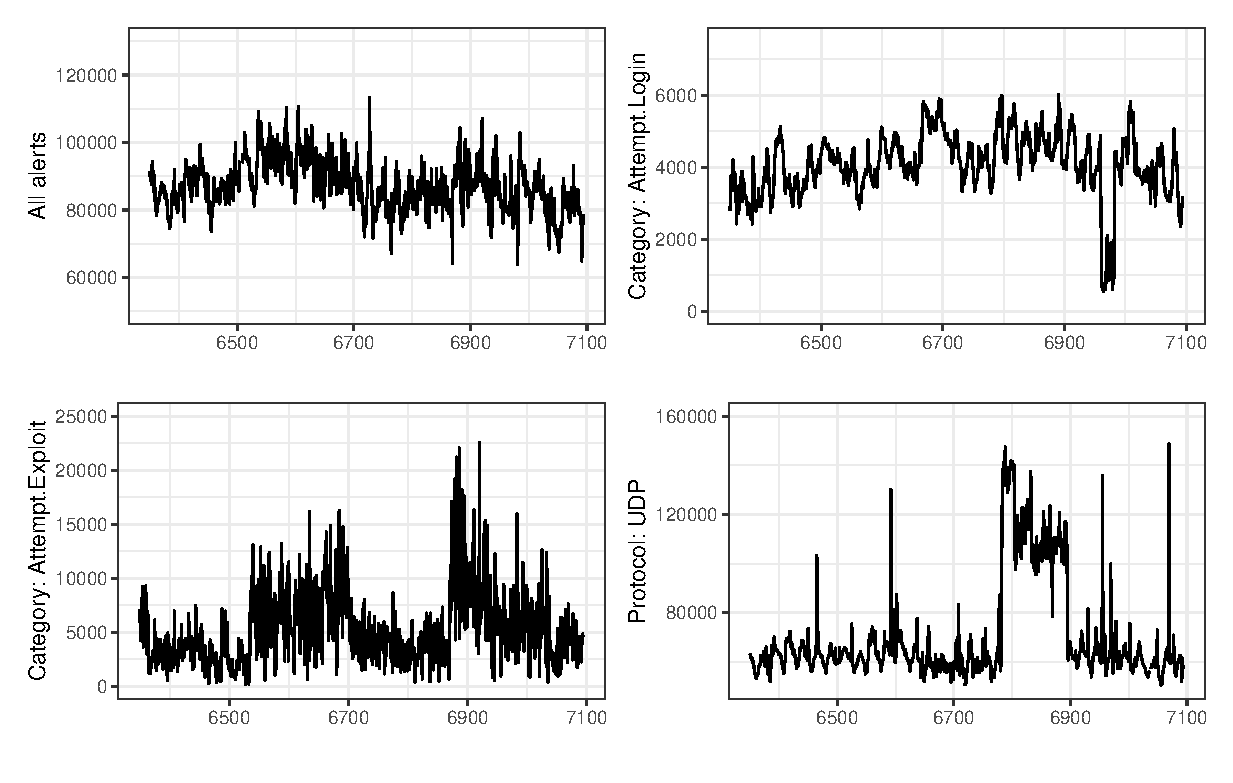
\includegraphics[width=0.9\textwidth]{images/TestFig3.eps}
  \caption{Náhľad časových radov za obdobie September 2018 a oblasti: All alerts - všetky udalosti; Category: Attempt.Login - Kategória pokus o~prihlásenie; Category: Attept.Exploit - Kategória pokus o~prienik; Protokol: UDP - Sieťový UDP protokol}
  \label{fig:timeseries_example}
\end{figure}

\section{Atribúty predikčných modelov}
V rámci prvého cieľa tejto práce sa venujeme výskumnej otázke \textit{Ako nájsť správnu kombináciu atribútov pre vylepšenie predikcie časových radov v~nepretržitej prevádzke?} príp. v~inom znení \textit{Ktoré atribúty je vhodné kombinovať pre zlepšenie predikcie časových radov v~nepretržitej prevádzke?}

Náš zdroj údajov poskytuje udalosti z~veľkého počtu rôznorodých senzorov. Senzory zbierajú údaje zo~sieťovej prevádzky, zo~zariadení (najmä zo~záznamov) ale aj zo~špeciálnych detekčných systémov - honeypotov. Problém, ktorý analyzujeme týmto cieľom je, predspracovanie vstupných údajov. Cieľom je zistiť, ktoré atribúty sú signifikantné pre identifikáciu útokov v~počítačovej sieti, tak aby sme ich predikciami dokázali upozorniť administrátorov o~zmenách situácie týchto sietí. Výskumnú otázku je možné formulovať aj nasledujúcim spôsobom: \textit{Ktoré parametre je vhodné kombinovať pre zlepšenie predikcie časových radov v~nepretržitej prevádzke? Aký vplyv má správny výber atribútov pre správnosť predikcií?}

%\textcolor{red}{- popis otázky, zavedenie definícii, 
% - rozvitie otázky, vysvetlenie, čo to znamená
%}
%1) Ktoré parametre (atribúty) sú kritické pre predikciu bezpečnostných udalostí/alertov používajúcu časové rady? Aký vplyv má na~úspešnosť predikcie výber vhodných parametrov? Ako ovplyvňujú tieto parametre výber vhodných časových radov? \\
% - tu by sa to rozbilo podľa typov predikcie s~tým, že už máš niečo k~security awareness

V podobných prácach oblasti kybernetickej bezpečnosti sa stretávame s~rôznymi dátovými sadami, s~akými výskumníci pracujú. Je však možné ich rozdeliť na~6 najčastejšie vyskytujúcich sa kategórií vypísaných v~tabuľke~\ref{tab:c1_datasets}. Keďže v~tejto práci sa venujeme predpovedaniu kybernetickej situácie v~počítačovej siete, tak pre komplexnú analýzu vhodných atribútov je dobré vedieť, aké výsledky nadobúdajú výskumníci aj z~menej (reputačných databáz - blacklist) príp. viac (sieťová prevádzka - PCAP) robustných dátových sád.

\begin{table}[]
    \centering
    \begin{tabular}{ | p{5cm} | p{9cm} | }
         \hline \textbf{Kategória} & \textbf{Príklady výskumných prác} \\
         \hline
         \hline Netflow & \cite{zang2019adaptive,fang2019deep,millar2019using,bakhshi2015user,jakalan2015profiling,marchette1999statistical,bernaille2006traffic,jirsik2020cyber} \\
         \hline Upozornenia \newline (IDS, Firewall) & \cite{granat2019big,werner2017time,shin2013advanced,ramaki2015real,soldo2011blacklisting} \\
         \hline Zraniteľnosti & \cite{tang2016exploiting,condon2008analysis,roumani2015time,tang2018disclosure,tang2017big,pokhrel2017cybersecurity} \\
         \hline PCAP & honeypots: \cite{zhan2015predicting,berti2017profiling,hammerschmidt2016efficient}; \newline simulácia siete \cite{jiang2004detecting}; \newline priemyselná bezdrôtová sieť: \cite{wei2012intrusion}  \\
         \hline Čierne zoznamy & \cite{liu2015cloudy} \\
         \hline Časový rad vyťaženia siete & \cite{cortez2012multi,hasegawa2001applications,papagiannaki2005long,sang2002predictability,wang2008internet} \\
         \hline
    \end{tabular}
    \caption{Rozdelenie dátových sád do~kategórií}
    \label{tab:c1_datasets}
\end{table}

\subsection{Aktuálny stav riešenej problematiky}

\subsubsection{Jednorozmerné časové rady}

Tabuľka~\ref{tab:ts_uni} zobrazuje prehľad využívaných atribútov časových radov v~podobných prácach. Autori experimentovali s~viacerými typmi údajov. Stretávame sa najmä s~troma atribútmi: (I) \textbf{veľkosť alebo počet paketov} v~sieťovej prevádzke, (II) \textbf{počet zraniteľností} a (III) \textbf{počet útokov}. Atribúty sú vo~väčšine prípadov najväčší všeobecne vytvorený časový rad z~dostupných údajov dátových sád. Napríklad z~IDEA udalostí získame počet útokov ako súčet všetkých údajov, z~dátovej sady net\-flow získame veľkosť prenesených paketov, prípadne ich počet a pod. Niekoľko autorov, ktorých spomenieme nižšie, sa hlbšie venujú dátovým sadám a časové rady rozdeľujú podľa aplikácií, protokolov alebo portov. 
Autori \cite{jiang2004detecting, wei2012intrusion,madan2018predicting, sang2002predictability,wang2008internet,hasegawa2001applications} pre svoj výskum predikcie situácie v~počítačovej sieti využili najzákladnejšie údaje. Údaje pozostávali z~dátového prenosu cez počítačové siete. Vo~väčšine prípadov dáta pochádzali z~produkčných sietí. Autori \cite{hasegawa2001applications} pre výskum použil prevádzkové dáta z~hlavného (backbone) spojenia medzi Spojenými štátmi americkými a Japonskom. Autori v~\cite{jiang2004detecting} vo~svojom výskume pristúpili k~viac kontrolovanému, simulovanému prostrediu. V~takom prostredí autori presne vedia, čo sa dialo a vďaka simulácii poznajú všetky vykonané útoky. V~dátach z~produkčných sietí môžeme mať veľký počet neodhalených útokov a mať skreslené informácie. Z~prevádzkových príspevkov vyčnieva \cite{wei2012intrusion}, ktorý namiesto bežných počítačových sietí analyzuje bezdrôtové priemyselné siete. Táto oblasť sa dnes spolu s~Internetom vecí (IoT) presadzuje stále viac, a preto si myslíme, že potvrdená aplikovateľnosť rovnakých princípov na~tieto siete je prínosom.

Autori v~\cite{cortez2012multi} rozdelili dostupné dátové sady na~3 rôzne kategórie. V~prvej sú dáta sieťovej prevádzky so~zjavnou sezónnosťou, v~druhej kategórii sú dáta s~viditeľnou periódou, avšak amplitúda v~periódach je náhodná a v~tretej kategórii sú dáta bez sezónnosti. Podľa publikovaného článku vo~všetkých kategóriách mali chybu predikcií časových radov v~rozmedzí 1 - 3~\%. Hasegawa vo~svojom článku \cite{hasegawa2001applications} porovnával rôzne veľkosti časových jednotiek 10 sekúnd, 30 sekúnd, respektíve 60 sekúnd. Tieto na~prvý pohľad malé časové jednotky získavajú väčší rozmer pri informácii o~produkčnom zdroji údajov, ktorým je hlavné spojenie (backbone) medzi Spojenými štátmi americkými a Japonskom. Zaujímavý prístup k~časovým radom je uvedený vo~výskume \cite{papagiannaki2005long}. V~tomto výskume autori pracujú so~špeciálnym posuvným oknom, kde znižujú váhu starších údajov. Môžu tak plynulo prechádzať na~nové údaje a zároveň pracovať s~pomerne veľkým oknom časových jednotiek.

Výskumná skupina Jiang a spol. vo~svojom výskume \cite{jiang2004detecting}  primárne využívali veľkosť prenesených paketov za časovú jednotku. V~rámci publikovaného článku píšu však o~testovaných alternatívnych časových radoch rozdelených podľa počtu komunikujúcich používateľov alebo podľa počtu paketov. Taktiež diskutujú o~možnosti rozdelenia časových radov podľa konkrétnych aplikácií, ako napríklad sharepoint - zdieľanie dokumentov, internet, ekonomické aplikácie a iné analyzovateľné aplikácie v~počítačovej sieti.

S ďalším veľmi zaujímavým prístupom prišli autori \cite{tang2016exploiting,roumani2015time,tang2018disclosure,tang2017big,pokhrel2017cybersecurity,werner2017time}. Vo~svojich prácach vytvárali časové rady z~počtu už zverejnených zraniteľností v~dostupných databázach, akou je aj Národná databáza zraniteľností (angl. National vulnerabilities database - NVD). Autor \cite{roumani2015time} využil prístup vnárania sa do~časových radov a vytvoril ich podľa viacerých atribútov: podla závažnosti, podľa postihnutých aplikácií, podľa úrovne zverejnených informácií a podobne.

Pri jednorozmerných časových radoch sa stretávame aj s~radmi reprezentujúcimi počet útokov za časové jednotky, \cite{zhan2015predicting} ako zdroj pre tieto časové rady využíva dátovú sadu obsahujúcu sieťovú prevádzku (PCAP) zo~siete honeypotov (honeynetu). Všetky spojenia smerujúce na~honeypoty označujeme za útoky, pretože na~honeypotoch nie je nasadzovaná legitímna komunikácia. Autor \cite{fang2019deep} prispel s~myšlienkou normalizácie časových radov počtu útokov, aby eliminoval extrémne hodnoty vyskytujúce sa v~prevádzkových sieťových udalostiach. Rovnako ako v~predchádzajúcich prístupoch, sa autor v~rámci~\cite{condon2008analysis} venuje možnosti použitia rôznych časových radov (podľa rôznych atribútov) namiesto jedného časového radu s~počtom útokov.

\begin{table}[]
    \centering
    \begin{tabular}{ | p{6cm} | p{8cm} | }
        \hline \textbf{Atribút} & \textbf{Príklady výskumných prác} \\
        \hline
        \hline veľkosť paketov & \cite{jiang2004detecting, wei2012intrusion,madan2018predicting, sang2002predictability,wang2008internet,hasegawa2001applications,cortez2012multi,papagiannaki2005long} \\
        \hline počet používateľov & \cite{jiang2004detecting} \\
        \hline počet paketov & \cite{jiang2004detecting} \\
        \hline počet paketov aplikácie \newline (samostatne) & \cite{jiang2004detecting} \\
        \hline počet zraniteľnosti & \cite{tang2016exploiting,roumani2015time,tang2018disclosure,tang2017big,pokhrel2017cybersecurity,werner2017time} \\
        \hline počet útokov \newline (z honeypotov a IDS systémov) & \cite{fang2019deep,zhan2015predicting,condon2008analysis} \\
        \hline
    \end{tabular}
    \caption{Atribúty jednorozmerných časových radov za časovú jednotku}
    \label{tab:ts_uni}
\end{table}

\subsubsection{Viacrozmerné časové rady}

Niekedy všeobecná informácia jednorozmerných radov nemusí byť postačujúca a generovala by len väčší šum, resp. nejednoznačnosť pri ich následnej interpretácii. V~takýchto prípadoch je pri predikciách zaujímavejšie pozrieť sa na~rozšírenú dátovú sadu (prezeranie do~šírky). Autori \cite{shin2013advanced,ramaki2015real,marchette1999statistical} sa rozhodli tento problém riešiť viacrozmernými časovými radmi, kde pre jednu časovú jednotku majú namiesto hodnoty vektor viacerých hodnôt podľa rôznych atribútov. Autor v~\cite{marchette1999statistical} pracoval s~údajmi netflow. Jedným z~atribútov sieťového toku netflow sú porty, na~akých zariadenia medzi sebou komunikujú. Z~tohto dôvodu jeho viacrozmerné rady vychádzali práve z~tohto atribútu. V~článku vybrali 1~\% najčastejšie sa vyskytujúcich portov do~viacrozmerného časového radu. Ďalší autor~\cite{roumani2015time} pracujúci s~bezpečnostnými udalosťami, ktoré boli v~dátovej sade kategorizované podľa využitých zraniteľností, sa rozhodol vytvoriť časové rady podľa tohto atribútu kategórií. Zaujímavý prístup publikoval autor v~\cite{shin2013advanced}, ktorý v~časových radoch vyjadroval entropiu zdrojových IP adries a portov, entropiu veľkosti paketov, početnosť paketov podľa atribútov (ICMP, UDP, TCP SYN) a tiež celkový počet paketov v~časovej jednotke.

%\begin{table}[]
%    \centering
%    \begin{tabular}{ | p{11cm} | p{3cm} | }
%        \hline IP + roznymi sposobmi agregovane netflow udaje, udajne pouzivaju aj delenie po kategoriach f http, p2p_other, DNS (48 udajov) & \cite{zang2019adaptive} \\
%        \hline agregovane podla IP/24 subnetov, pouzivaju well-known porty a protokoly (najmä 139, 1433, 443, 445) & \cite{soldo2011blacklisting} \\
%        \hline orezane flow data na~prvych 50 bytov (rozdelene po kategoriach DOS, EXPLOITS, FUZZERS, GENERIC, RECONNAISSANCE, OTHER-MALICIOUS, NON-MALICIOUS, Total) & \cite{millar2019using} \\
%        \hline flowy vytvorene podla hostov (userov) & \cite{bakhshi2015user} \\
%        \hline sucet peerov, ratio roznych paketov v~portadi, ratio destination portov, rozne entropie a pod. & \cite{jakalan2015profiling} \\
%        \hline ip, dest. port, header length, udp length, dont fragment flag, TTL, Corrupted & \cite{berti2017profiling} \\
%        \hline protocol, time, duration, packet, data exchanges, data received & \cite{hammerschmidt2016efficient} \\
%        \hline 
%    \end{tabular}
%    \caption{PARAMETRE nie TS - profilacia}
%    \label{tab:my_label}
%\end{table}

\subsection{Prístup k~riešeniu výskumného cieľa} \label{c1_metodologia}

Ako sme popísali v~úvode tejto kapitoly, v~práci pracujeme s~dátovou sadou od~českej akademickej siete CESNET. Dátová sada obsahuje udalosti v~IDEA formáte. V~prvom rade sme urobili analýzu tejto dátovej sady, aby sme získali bližší prehľad o~početnosti udalostí v~jednotlivých kategóriách, sieťových portoch, protokoloch a výraznej existencii ďalších atribútov. Pri úvodných analýzach zozbieraných údajov sa zistila nevhodnosť ich uloženia vo~veľkej SQLite databáze bez akýchkoľvek indexov. Spôsob uloženia doteraz zozbieraných údajov sme upravili tak, aby databáza obsahovala udalosti v~rovnakom poradí, v~akom boli prijaté. Nový spôsob nebude vytvárať jednu veľkú databázu IDEA udalostí. S~veľkou databázou sa spájajú viaceré analytické, ale aj distribučné problémy. Preto sme nastavili obmedzenie na~jednu SQLite databázu na~jeden kalendárny deň. Získali sme tak síce veľa malých (1 - 3~GB) súborov, ale bez výkonnostných problémov dokážeme údaje prehrávať aj distribuovať ďalším výskumníkom za akokoľvek dlhé obdobie. 

Tvorbu časových radov budeme vykonávať prehraním dátovej sady cez agregačný algoritmus. Tento algoritmus za každú minútu spočíta udalosti podľa zvolených výz\-namných kritérií a súčty uloží do~databázy pre danú časovú jednotku. Prehranie dátovej sady prebieha cez technológiu posielania správ Apache Kafka a za databázu pre uloženie časových radov sme zvolili PostgreSQL s~rozšírením pre efektívnu prácu s~časovými radmi TimescaleDB. Prístup posielania správ je zvolený z~dôvodu podpory neustáleho príjmu údajov. Pre spustenie rovnakého systému v~reálnej prevádzke budeme potrebovať len presmerovať zber IDEA udalostí zo~systému WARDEN do~našej inštancie Apache Kafka. Na~schéme č.~\ref{fig:c1_schema} je vizuálne znázornené fungovanie navrhovaného riešenia.

\begin{figure}[h]
  \centering
  \includegraphics[width=0.9\textwidth]{images/metodologia1.png}
  \caption{Schéma od~zberu údajov cez internú distribúciu po spracovanie časových radov v~troch samostatných službách}
  \label{fig:c1_schema}
\end{figure}

Okrem doteraz získavaných údajov z~dátovej sady je potrebné venovať sa aj doplneniu informácií (obohatenie dátovej sady). Za externé informácie považujeme napríklad databázu zraniteľností. Tá bude tvoriť ďalšie časové rady a môže zvyšovať citlivosť predikčných algoritmov. Okrem zraniteľností vieme doplnením rozšírených informácií k~IP adresám vytvoriť ďalšie časové rady zohľadňujúce spojenia s~konkrétnymi krajinami, prípadne poskytovateľmi internetového pripojenia (ISP).

\section{Vhodnosť predikčných modelov}
V druhom cieli tejto práce sa bližšie venujeme výskumnej otázke \textit{Ktoré predikčné modely sú vhodné pre využitie v~nepretržitej prevádzke?}

V tejto práci sa venujeme najmä predpovedi situácie v~počítačových sieťach. Dátovú sadu tohto čiastkového cieľa už máme v~podobe jedno- aj viacrozmerného časového radu. Od~dátovej sady tiež očakávame jej neustále generovanie a potrebujeme uvažovať aj nad jej časovou náročnosťou, aby pri využívaní predikčných modelov nenastali časové sklzy v~predikciách a príjme nových údajov. Hlavným cieľom témy tejto práce podľa rozdelenia z~kapitoly \ref{discipliny} je predikcia kybernetickej situácie v~počítačovej sieti, bližšie definovaná v~\ref{forecast}.


% 2) Ktoré z~ML modelov sú vhodné pre predikciu v~reálnom čase? How do~variations in the model’s training period affect the performance? Can we reuse a trained model for a given period of time and when do~we need to retrain the model? Ako ovplyvňujú pamäťové nároky jednotlivých modelov dosiahnutie predikcie bezpečnostných udalostí/alertov v~reálnom čase?\\
%  - delene metód na~predikciu - podľa typov (ako to má M. Husák)\\
%  - sezónnosť, časové okná\\
%  - krátkodobé, dlhodobé predikcie a pod.\\
%  - aké metódy používajú v~článkoch\\ 
%  - aké sú kritéria pre on the fly alebo real-time predikciu\\

\subsection{Aktuálny stav riešenej problematiky}

Analýzou dostupnej literatúry k~oblasti predikcie situácie v~kybernetickej bezpečnosti sme dospeli k~rozdeleniu na~3 oblasti použitých metód:
\textbf{štatistické metódy}, \textbf{neurónové siete} a ďalšie metódy. 

Prehľad použitých metód podľa tohto rozdelenia je zobrazený v~tabuľke č.~\ref{tab:c2_alg}. Aktuálne najvýznamnejšou oblasťou sú štatistické metódy. V~posledných rokoch je možné pozorovať nárast výskumnej aktivity v~oblasti neurónových sietí. Obe tieto oblasti sú vhodné na~porovnanie s~výsledkami našej výskumnej práce a potvrdenie využitia týchto metód pre spracovanie v~nepretržitých prevádzkach. Našli sme aj práce využívajúce klasifikačné metódy v~reálnom čase na~klasifikovanie sieťovej prevádzky a filtrovaniu veľkého počtu dát podľa správania útočníkov. Tieto dáta sú zaujímavým prístupom, ako pomocou klasifikačných metód odhaliť podvodné aktivity a zlepšiť informovanosť o~aktuálnej situácii v~počítačovej sieti.

\begin{table}
    \centering
    \begin{tabular}{ | p{6cm} | p{4cm} | p{4cm} | }
         \hline \textbf{Metóda} & \textbf{Príklady\newline výskumných prác} & \textbf{Použité atribúty} \\

         \hline \multicolumn{2}{l}{\textbf{Štatistické metódy}} \\
         % ARIMA rodina
         \hline ARIMA & \cite{madan2018predicting,papagiannaki2005long,condon2008analysis,roumani2015time,tang2018disclosure,tang2017big,pokhrel2017cybersecurity,werner2017time,cortez2012multi} & VP, PZ, PÚ \\
         \hline ARMA & \cite{wei2012intrusion,sang2002predictability} & VP \\
         \hline SARIMA & \cite{tang2016exploiting,condon2008analysis,roumani2015time,tang2018disclosure} & PZ, PÚ \\
         \hline FARIMA & \cite{zhan2015predicting} & PÚ \\
         % ARCH rodina
         \hline GARCH & \cite{tang2016exploiting,tang2018disclosure,tang2017big} & PZ \\
         % holt winters rodina
         \hline Holt-Winters & \cite{cortez2012multi,roumani2015time} & VP, PZ \\
         \hline Local Linear Approximation (LLA) & \cite{hasegawa2001applications} & VP \\
         \hline EWMA - Exponential Weighted Moving Average & \cite{soldo2011blacklisting} & firewall logy \\

         
         
         % neuronkovy pristup
         \hline \multicolumn{2}{l}{\textbf{Neurónové siete}} \\
         \hline Neurónové siete & \cite{Leau2015,wang2008internet} & VP \\
         \hline Rekurentné neurónové siete & \cite{madan2018predicting,fang2019deep} & VP, PÚ \\
         \hline Dopredné neurónové siete & \cite{cortez2012multi,pokhrel2017cybersecurity} & VP, PZ \\
         \hline Konvolučné neurónové siete & \cite{millar2019using} & Netflow \\
         \hline LSTM neurónové siete & \cite{fang2019deep} & PÚ \\
         
         % klasifikacna
         \hline \multicolumn{2}{l}{\textbf{Ostatné}} \\
         \hline Random Forrest (RF) & \cite{liu2015cloudy} & VP \\
         \hline Support vector machine (SVM) & \cite{liu2015cloudy,hasegawa2001applications,Leau2015,pokhrel2017cybersecurity} & VP, PZ \\
         %\hline K najbližších susedov (KNN) & \cite{soldo2011blacklisting,shin2013advanced,marchette1999statistical} \\
         %\hline K - Means &\cite{bakhshi2015user,berti2017profiling,hammerschmidt2016efficient,bernaille2006traffic} \\
         %\hline DBSCAN & \cite{jakalan2015profiling,berti2017profiling} \\
         %\hline Prefix tree acceptor (PTA) & \cite{hammerschmidt2016efficient} \\
         %\hline Bayesan attack graph (BAG) & \cite{ramaki2015real} \\
         
         %\hline Event Strength Function (ESF) & \cite{granat2019big} \\
         %\hline Multi - Dynamic pareto set & \cite{granat2019big} \\
         %\hline Radial basis functuin (RBF) & \cite{hasegawa2001applications,wang2008internet} (wang optimalizuje genetickym alg.) \\
         
         %\hline Markov model & \cite{shin2013advanced,sang2002predictability} \\
         %\hline 
         % v~texte \hline Wavelet (discrete + multiresolution) tranformacia & \cite{madan2018predicting,papagiannaki2005long} \\
         % v~texte \hline kobinacia ARIMA + RNN & \cite{madan2018predicting} \\
        
         \hline
    \end{tabular}
    \caption{Prehľad algoritmov v~dostupnej literatúre s~atribútmi, aké použili (podľa tab. \ref{tab:c1_datasets}). VP - veľkosť paketov, PZ - počet zraniteľností, PÚ - počet útokov.}
    \label{tab:c2_alg}
\end{table}

V oblasti štatistických metód urobili prehľad autori článku \cite{roumani2015time}. Na~predikcie využívali dátovú sadu zraniteľností v~časových radoch, rozdelenú podľa aplikácií. Pre každú aplikáciu, ale aj pre celkový časový rad testovali vhodnosť metód ARIMA a Holt-Winters. Taktiež testovali metódu sezónnej verzie ARIMA metódy (SARIMA). Vo~svojej práci prezentujú najmenšiu percentuálnu chybu 12~\%. Autor \cite{tang2018disclosure} študoval ARCH efekt údajov na~zraniteľnostiach pomocou rôznych GARCH modelov (generalizovaný ARCH). Autor výskumu tvrdí, že najlepším modelom pre údaje počítačových zraniteľností je sGARCHstd(1,1), s~overením pomocou Akaikeho informačného kritéria (AIC) a Bayesovho informačného kritéria (BIC).

Autori \cite{madan2018predicting,papagiannaki2005long} pridali pred využitie ARIMA metódy wavelet transformáciu~\cite{torrence1998practical} do~frekvenčného spektra. Využitím už spomenutej wavelet transformácie sa im podarilo eliminovať dlhodobo rastúci trend vyťaženosti hlavnej (backbone) prevádzky. Autor \cite{madan2018predicting} okrem wavelet transformácie vykonal svoje predikcie aj spojením metódy ARIMA a Rekurentnej neurónovej siete. Výsledná predikcia ďalšej časovej jednotky je v~jeho článku prezentovaná ako kombinácia predikcií oboch metód. Autor v~rámci práce \cite{tang2016exploiting} porovnal vhodnosť využitia metód ARIMA a GARCH na~dátovej sade zraniteľností. V~práci uvádzajú ARCH efekt a tvrdia, že GARCH metódy predpovede dávajú lepšie výsledky na~ich dátovej sade.

Cortez a spol. vo~svojej práci~\cite{cortez2012multi} využili predikcie pomocou metód ARIMA a Holt-Winters ako referenciu pre plne prepojenú viacvrstvovú neurónovú sieť s~počtom uzlov od~1 do~289. Vo~výsledkoch prezentujú zlepšenie predikcií oproti referenčným ARIMA a Holt Winters modelom o~0,4~\%. Podobnému porovnaniu sa venujú aj autori článku \cite{fang2019deep}. Referenčné výsledky z~ARIMA modelu porovnávajú s~rekurentnými neurónovými sieťami (RNN) s~LSTM neurónmi. Vo~svojej práci navrhli obojsmernú rekurentnú neurónovú sieť s~LSTM neurónmi pre predikcie budúceho správania počítačovej siete. Výsledky ich experimentu na~dátovej sade netflow sa však prikláňajú k~štatistickým metódam ARIMA. V~diskusii autor uvádza iné spôsoby vytvorenia siete obsahujúcej viac ako 4 LSTM neurónov, s~potenciálne lepšími výsledkami. Ďalšie zaujímavé riešenie prináša článok \cite{millar2019using}, v~ktorom sa dočítame o~využití konvolučných neurónových sietí pre profilovanie sieťových spojení zo~sieťových údajov (netflow). Vstupom do~neurónovej siete je prvých 50 bajtov z~netflow záznamu. Autori článku \cite{soldo2011blacklisting} po odhalení, že veľký počet útočiacich IP prefixov závisí od~blízkej minulosti, použili metódu exponenciálneho a váženého kĺzavého priemeru. V~experimente porovnali svoje výsledky s~Cross-Association metódou a predikcie s~kĺzavým priemerom ukázali o~25~\% lepšie výsledky.

Leau vo~svojom článku~\cite{Leau2015} analyzoval vhodnosť použitia neurónových sietí, Markovského modelov a Gray Theory modelov pre predikovanie situácie v~kybernetickej bezpečnosti. V~zhrnutí píše najmä o~dôležitosti a robustnosti trénovacej dátovej sady pre neurónové siete aj Markovského modely. Často nedostatočné dátové sady spôsobujú vysoké percento chyby týchto modelov. Napriek tomu tvrdí, že Gray Theory môže poskytnúť dobré predikcie s~malou vstupnou dátovou sadou, a to bez nutnosti trénovania.

Autori v~článku~\cite{shin2013advanced} navrhli nový spôsob klasifikácie situácií v~kybernetickej bezpečnosti nazvaný APAN (angl. Advanced Probabilistic Approach for Network-based IDS). Tento spôsob označí aktuálny stav v~počítačovej sieti jednou z~piatich rizikových kategórií ({red, orange, yellow, blue, green}). Prístup sa skladá z~troch fáz: (1) vykoná sa K-means klastrovanie so~zohľadnením outlierov, (2) je vytvorený Markovského model s~prechodovou maticou podľa klastrov, (3) v~reálnom čase sa vyhodnotí rizikovosť aktuálnej prevádzky. Autori \cite{liu2015cloudy} analyzovali použiteľnosť Random Forest (RF) metódy pre predpovedanie kybernetickej situácie s~90~\% úspešnosťou detekcie podvodnej prevádzky. Svoje výsledky porovnali s~metódou Support Vector Machine (SVM), kde úspešnosť detekcie nepresiahla 70~\%. Pri RF metóde poukazujú len na~10~\% false-negatives v~experimentoch.

\subsection{Prístup k~riešeniu výskumného cieľa}\label{c2_metodologia}

Pre prácu v~nepretržitej prevádzke je výhodnejšie využiť metódy s~automatickým učiacim procesom. Takéto metódy sú navrhnuté tak, aby automaticky vyberali najlepší model. Učiace modely predikcií sa objavujú v~rôznych nastaveniach. Pod nastaveniami rozumieme zlepšenú podporu pre sezónnosť vstupných údajov a spôsob, akým budú údaje prichádzať do~predikčných modelov. Analyzujeme 2 spôsoby učenia modelu. V~prvom, klasickom prístupe do~modelu postupne vkladáme hodnoty ďalších časových jednotiek z~trénovacej sady. V~druhom spôsobe využívame tzv. posuvné okno, čo znamená, že predikčný algoritmus vždy vidí rovnako veľkú vstupnú dátovú sadu. Vždy po prijatí novej časovej jednotky je najstaršia časová jednotka odstránená. V~tomto spôsobe sme schopní udržiavať rozumnú veľkosť vstupu predikcií pri použití v~nepretržitej prevádzke.

Ako prvé overenie nového modelu počítame pomocou 95~\% predikčného intervalu (bootstrap). Následne sa vypočíta priemerné pokrytie. Priemerné pokrytie je percento spoľahlivosti intervalov, ktoré správne pokryli skutočné hodnoty časového radu. Percento by malo byť v~okolí 95~\%, pretože potom sú predikcie vhodné pre konkrétny prípad (t. j. pre metódu, počet predikcií do~budúcnosti a časový interval). Nižšie pokrytie ako 95~\% by znamenalo horšiu spoľahlivosť predikčného intervalu a vyššie pokrytie ako 95~\% znamená širší a menej informatívny interval.

V práci tiež zohľadňujeme priemernú dĺžku predikčných intervalov. Vo~všeobecnosti sa kratšie predikčné intervaly považujú za presnejšie. Dávajú nám lepšie informácie o~budúcich hodnotách časových radov. Naše hodnotenie rozdelíme do~dvoch fáz. V~prvej fáze budeme hodnotiť metódy predpovedí iba na~základe celkového počtu upozornení a nebudeme zohľadňovať kvalitatívnu zložku (kategória výstrah, sieťový port alebo sieťový protokol). Výskum je založený na~výsledkoch z~článku~\cite{new_paper}, v~rámci ktorého sa autori venovali 24-hodinovým obdobiam a štyrom rôznym časovým jednotkám (5 minút, 15 minút, 30 minút a 60 minút) a veľkosťou dátovej sady obsahujúcej bezpečnostné udalosti zozbierané počas jedného týždňa. V~tejto práci rozširujeme tento príspevok o~zložku neustáleho príjmu údajov. Dôležitá je tiež skutočnosť, že k~dispozícii máme väčšie obdobie udalostí. Pre účely čiastkových výsledkov sme spracovali ročné údaje. Na~základe predchádzajúcej práce sme sa rozhodli pracovať s~24-hodinovými a 7-dňovými obdobiami s~dvoma rôznymi časovými jednotkami (30 minút a 60 minút) a dvoma rôznymi dĺžkami dátovej sady (1 mesiac a 2 mesiace). Hlavným cieľom tejto fázy je odpovedať na~otázky sezónnosti a používania posuvných okien v~perspektíve dlhodobého obdobia (jeden rok).

V druhej fáze našej evaluácie používame najlepšiu kombináciu časového intervalu, periódy a predpovedného obdobia (30 minút, 7 dní, jeden mesiac). V~tejto fáze vyhodnocujeme metódy predpovedania 21 atribútov udalostí a zaoberáme sa kvalitatívnou zložkou (kategória udalostí, sieťový port alebo sieťový protokol). Hlavným cieľom tejto fázy je analyzovať sezónnosť a využitie posuvných okien v~iných časových radoch s~prihliadnutím na~kvalitatívnu zložku. Analyzujeme kritéria ovplyvňujúce predpovedanie (forecasting) použitím časových radov.


\begin{figure}[h]
  \centering
  \includegraphics[width=0.9\textwidth]{images/metodologia2.png}
  \caption{Architektúra distribúcie časových radov do~modelov.}
  \label{fig:c2_schema}
\end{figure}


Architektúra riešenia tohto cieľa je znázornená na~obrázku č.~\ref{fig:c2_schema}. Na~vstupe predikcií je neustále vytváraný a ukladaný časový rad. Rad je pri uložení znova distribuovaný pomocou platformy Apache Kafka, kde môžeme mať niekoľko inštancií predikčných modelov postavených na~rôznych časových radoch.

\section{Presnosť predikčných modelov}
V tomto cieli práce hľadáme odpovede na~výskumnú otázku \textit{Ako vyhodnocovať presnosť predikčných modelov na~dátach kybernetickej bezpečnosti? Aké metriky sú vhodné pre tieto modely?}

Dôležitosť vyhodnotenia presnosti predikčných modelov spočíva v~porovnaní viacerých modelov. Vyhodnotením zisťujeme, či nové modely dosahujú lepšie alebo horšie výsledky oproti existujúcim modelom. Pre porovnanie však potrebujeme matematický model (označujeme ho aj metrika), ktorý vypočíta celkovú chybu vypočítaných pre\-dikcií. Existuje však množstvo spôsobov na~výpočet chyby a nie je možné genericky pre každý prípad vybrať ten najlepší. 

\subsection{Aktuálny stav riešenej problematiky}

Výber metódy pre výpočet chyby závisí priamo od~dátovej sady, s~ktorou pracujeme a tiež od~očakávaní od~našich predikcií. Spôsoby, akými môžeme merať chybu v~predikciách, sú podľa~\cite{hyndman2018forecasting}:  \textbf{chyby závislé od~rozsahu}, \textbf{percentuálne vyjadrené chyby},  \textbf{škálované chyby}. V~tabuľke č.~\ref{tab:c3_metrics} je prehľad metrík, s~akými sa stretávame v~dostupnej literatúre aj s~uvedením zápisu konkrétnych metrík. V~zápise metrík $y_t$ je pozorovaná/nameraná hodnota, $\hat{y}_{t}$ je odhad hodnoty a $n$ prislúcha celkovému počtu hodnôt, z~ktorých sa metrika počíta.

\begin{longtable}[p]{ | p{4cm} | p{5.5cm} | p{4.5cm} | }
    \caption{Prehľad použitých metrík v~literatúre.}
    \label{tab:c3_metrics}\\
    \hline \textbf{Metrika} & \textbf{Zápis} & \textbf{Použitie v~literatúre}\\
    \endfirsthead
    \hline \textbf{Metrika} & \textbf{Zápis} & \textbf{Použitie v~literatúre}\\
    \endhead
     \hline \textbf{MAE} - Mean Absolute Error & $${{\frac {\sum _{t=1}^{n}\left|y_{t}-\hat{y}_{t}\right|}{n}}}$$ & \cite{tang2018disclosure} \\
     \hline \textbf{RSME} - Root Mean Square Error & $${{\sqrt {\frac {\sum _{t=1}^{n}({y}_{t}-\hat{y}_{t})^{2}}{n}}}}$$ & \cite{tang2018disclosure,tang2017big,condon2008analysis} \\
     \hline \textbf{MAD} - Mean Absolute Deviation & $${{\frac {1}{n}}\sum _{t=1}^{n}{\left|{y_{t}-{\hat {y}}_{t}}\right|}}$$ & \cite{fang2019deep} \\
     \hline \textbf{MSE} - Mean Square Error & $${{\frac {1}{n}}\sum _{t=1}^{n}(y_{t}-{\hat {y_{t}}})^{2}.}$$ & \cite{fang2019deep,werner2017time} \\
     \hline \textbf{NMSE} - Normalized Mean Square Error & $$\frac{n\cdot\sum _{t=1}^{n}\left|y_{t} - \hat{y}_{t}\right|^{2}}{\sum _{t=1}^{n}{y_{t}} \cdot \sum _{t=1}^{n}{\hat{y}_{t}}}$$ & \cite{zang2019adaptive,madan2018predicting} \\
     \hline \textbf{SSE} - Sum Squared Error & $${\sum _{t=1}^{n}(y_{t}-\hat{y}_{t})^{2}}$$ & \cite{cortez2012multi} \\
    
     \hline \textbf{MAPE} - Mean Absolute Percentage Error & $${\frac  {1}{n}}\sum _{{t=1}}^{n}\left|{\frac  {y_{t}-\hat{y}_{t}}{y_{t}}}\right|$$ & \cite{jiang2004detecting,cortez2012multi,fang2019deep,tang2018disclosure,werner2017time} \\
     \hline \textbf{SMAPE} - Symetric Mean Absolute Percent Error & $${\frac {100\%}{n}}\sum _{t=1}^{n}{\frac {\left|y_{t}-\hat{y}_{t}\right|}{(|y_{t}|+|\hat{y}_{t}|)/2}}$$ & \cite{roumani2015time,pokhrel2017cybersecurity} \\
     \hline \textbf{PMAD} - Percent Mean Absolute Deviation & $${\frac {\sum _{t=1}^{n}\left|y_{t}-{\hat {y}}_{t}\right|}{\sum _{t=1}^{n}\left|y_{t}\right|}}$$ & \cite{fang2019deep,zhan2015predicting} \\
     
     \hline \textbf{BIC} - Bayesian Information Criterion & $${n\ln({\frac {1}{n}}\sum _{t=1}^{n}({y_{t}-{\widehat {y_{t}}})^{2}})+k\ln(n)\ }$$ & \cite{tang2016exploiting} \\
     \hline \textbf{AIC} - Akaike Information Criterion & $${2k-2\ln({\hat {L}})}$$ & \cite{tang2016exploiting,zhan2015predicting,wei2012intrusion} \\
     \hline

\end{longtable}

Pre chyby závislé od~rozsahu platí, že sú v~rovnakom rozsahu (škále) ako dátová sada. Preto takto vypočítaná chyba nemôže byť použitá v~dátových sadách obsahujúcich rôzne jednotky. Dve najčastejšie používané metriky závislé od~škály sú založené na~absolútnych hodnotách chyby alebo na~druhej mocnine chyby. Medzi tieto metriky patria aj MAE a RMSE. Napriek tomu, že RMSE je zložitejšou metrikou, pomerne často sa využíva \cite{tang2018disclosure,tang2017big,condon2008analysis}. 

Výhody percentuálne vyjadrených chýb, najčastejšie pomocou metriky MAPE, využívajú vo~svojom výskume autori \cite{jiang2004detecting,cortez2012multi,fang2019deep,tang2018disclosure,werner2017time}. V~oblasti kybernetickej bezpečnosti metriku SMAPE, ktorá rieši neadekvátne tresty za záporné hodnoty, využívajú autori v~rámci prác \cite{roumani2015time,pokhrel2017cybersecurity}.

Ďalšou metódou, ktorá sa výraznejšie vyskytuje v~podobných prácach \cite{tang2016exploiting,zhan2015predicting,wei2012intrusion}, je Akaikeho informačné kritérium (AIC), ktoré odmeňuje dobrú predpoveď. Zahŕňa však aj pokutu, ktorá je zvyšujúcou sa funkciou počtu odhadovaných parametrov. Pokuta zamedzuje nadmerné učenie, ktoré je nežiaduce, pretože zvýšenie počtu parametrov v~modeli takmer vždy zlepšuje kvalitu predpovedí, ale zvyšuje časovú náročnosť. Podobný prístup ako AIC prináša aj Bayesove informačné kritérium (BIC), v~ktorom je vyššia pokuta za nadmerné učenie. Tento prístup spolu s~AIC využili v~článku \cite{tang2016exploiting}.

% 3) How to evaluate real-time predictions in cyber security and what metrics should be used? What is proposed system performance in identifying the upcoming security events/alerts and how does its performance compare to the baseline and state-of-the-art methods? Is it sufficient to rely on evaluation using datasets and testbeds or can the actual prediction accuracy be measured in a live network setting? \\
%  - porovnať metódy (všeobecne) \\
%  - porovnať metódy použité v~článkoch - napr. ktoré metódy sa pri akých údajoch, akých typoch predikcií používajú \\
%  - pozrieť diskusie v~článkoch - postačujú len datasety? Ako porovnávať s~inými údajmi \\
%  - urobit porovnanie metrik \\

\subsection{Prístup k~riešeniu výskumného cieľa}
 
Vyhodnotenie kvality predpovedí vybraných modelov budeme robiť pomocou krížovej validácie~\cite{hyndman2018forecasting}. Použijeme dve variácie tohto prístupu. V~prvom prípade vypočítame predpovede v~konkrétnych budúcich časoch (osobitne pre jeden, dva, päť alebo desať krokov do~budúcnosti) testovacej sady a na~konci vypočítame metrickú hodnotu zo~všetkých predpovedí osobitne pre rôzne predikčné kroky. V~druhom prípade krížovej validácie budeme zvažovať všetky prognózy až do~druhého, piateho a desiateho kroku predpovede. V~oboch variáciách vypočítame hodnotenie presnosti rovnakou metrikou.

V rámci budúcej práce tento postup zopakujeme s~rôznymi dátovými sadami (podľa metodológie~\ref{c1_metodologia}), modelmi (podľa metodológie~\ref{c2_metodologia}) a metrikami z~tejto podkapitoly. Pri výbere použitej metriky budeme na~základe podobných prác uvažovať nad ich použiteľnosťou na~našu dátovú sadu. Dôležitými parametrami pre použitie sú rovnaké jednotky pri prvej skupine, prípadne rôzne jednotky pri percentuálnej skupine metrík. Pri percentuálnych nemôžeme zabudnúť na~obmedzenie pri veľmi malých hodnotách, ktoré by mohli viesť k~nedefinovaným alebo nekonečným výsledkom.

\chapter{Parciálne výsledky}

% Doposiaľ sme sa nevenovali zahrnutím externých údajov, ktoré plánujeme v~najbližšom období. 
Spracovali sme vyššie uvedenú dátovú sadu do~časových radov podľa metodológie~\ref{c1_metodologia}. Vytvorené časové rady sú uložené v~PostgreSQL databáze a pripravili sme z~nich viac verzií agregovaných po jednej minúte, desiatich minútach, pätnástich minútach, tridsiatich minútach a šesťdesiatich minútach. Takéto rady sme vytvorili pre každý z~21 zvolených atribútov: (1) Počet všetkých udalostí, (2) Počet unikátnych IP adries, (3)  Kategória skenovanie zariadenia, (4) Kategória preťaženie služby DDoS (angl. Denial of service), (5) Kategória pokus o~prihlásenie, (6) Kategória pokus o~zneužitie, (7) Kategória malware / ransomware, (8) Kategória prienik botnetu, (9) Port 21, (10) Port 22, (11) Port 23, (12) Port 25, (13) Port 80, (14) Port 443, (15) Port 445, (16) Protokol TCP (angl. Transmission Control Protocol), (17) Protokol SSH (angl. Secure Shell), (18) Protokol UDP (angl. User Datagram Protocol), (19) Protokol ICMP (angl. Internet Control Message Protocol), (20) Protokol Microsoft WBT Server (angl. Windows-Based Terminal), (21) Protokol Telnet.

Pripravenú dátovú sadu časových radov sme exportovali do~súborov vo formáte csv (comma-separated values), aby sme ich mohli analyzovať v~jazyku R a v~jednej z~najrozšírenejších knižníc pre predikcie časových radov nazývanej Forecast r-package~\cite{hyndman2007automatic}. Pre prácu v~nepretržitej prevádzke je výhodnejšie využiť metódy s~automatickým učiacim procesom. V~spomenutom R rozšírení k~takým patrí ARIMA alebo ETS. Tieto metódy sú navrhnuté tak, aby automaticky vybrali najlepší model, ktorý bude zohľadňovať zadanú metriku~\cite{hyndman2007automatic}.

Pre každú triedu modelov boli konkrétne modely testované v~sezónnom a ne-sezónnom nastavení. Rozhodli sme sa vybrať posledné dva mesiace z~celého jednoročného súboru údajov z~dôvodu časovej zložitosti našej rozsiahlej predikčnej štúdie. Je možné predpokladať, že hodnoty časových radov v~minulosti (pokiaľ ide o~časové jednotky) by nemali výrazný vplyv na~predpovede budúcich hodnôt. Zvažovali sme 2 spôsoby učenia modelu, uvedené v~metodológii~\ref{c2_metodologia}, klasický model a model s~tzv. posuvným oknom. Pre účely čiastkových výsledkov prvej fázy sme sa rozhodli pracovať s~24-hodinovými a 7-dňovými obdobiami s~dvoma rôznymi časovými jednotkami (30 minút a 60 minút) a dvoma rôznymi dĺžkami dátovej sady (1 mesiac a 2 mesiace). V~druhej fáze našej evaluácie čiastkových výsledkov používame najlepšiu kombináciu časového intervalu, periódy a predpovedného obdobia (30 minút, 7 dní, jeden mesiac). V~tejto fáze vyhodnocujeme metódy predpovedania 21 atribútov udalostí a zaoberáme sa kvalitatívnou zložkou (kategória udalostí, sieťový port alebo sieťový protokol).

V nasledujúcich sekciách podrobnejšie opisujeme obe fázy vyhodnotenia experimentu. Podrobnejšie sa pozrieme na~jednotlivé výsledky a na~základe nich diskutujeme o~čiastkových otázkach.

%-------------------------------------------------------
% The first stage - results
%-------------------------------------------------------
\section{Prvá fáza predikcií časových radov}

V rámci hodnotenia sme v~prvej fáze testovali všetky vyššie uvedené metódy v~šiestich prípadoch (časový interval, časové obdobie, časová jednotka): 
\begin{compactenum}
    \item 30 minút, 24 hodín, 1 mesiac; 
    \item 30 minút, 7 dní, 1 mesiac; 
    \item 60 minút, 24 hodín, 2 mesiace; 
    \item 60 minút, 24 hodín, 1 mesiac; 
    \item 60 minút, 7 dní, 2 mesiace; 
    \item 60 minút, 7 dní, 1 mesiac.
\end{compactenum}



% ------------- cross-validation  -----------------------------

Prvým prístupom na~vyhodnotenie kvality predpovedí konkrétnych modelov je tzv. krížová validácia~\cite {hyndman2018forecasting}. Použili sme dve variácie tohto prístupu. V~prvom prípade sme vypočítali predpovede v~konkrétnych budúcich časoch (osobitne pre jeden, dva, päť alebo desať krokov do~budúcnosti) testovacej sady a na~konci sme vypočítali metrickú hodnotu zo~všetkých predpovedí osobitne pre rôzne predikčné kroky. Použili sme metriku priemerná absolútna miera chybovosti (MASE)~\cite{hyndman2006another}, často používanú na~vyhodnotenie presnosti prognózy. Túto metriku uprednostňujeme vďaka tomu, že je menej citlivá na~odľahlé hodnoty, ľahšie interpretovateľná a menej variabilná na~malých vzorkách.

Metrika MASE je definovaná ako~\cite{hyndman2018forecasting}:

% 
\begin{equation}
\textrm{MASE} = \textrm{mean}(|q_j|)
\end{equation}
% 
kde $q_j$ pre časové rady bez sezónnosti je:
% 
\begin{equation} 
q_j= \frac{e_j}{\frac{1}{T-1} \sum_{i=2}^{T}|y_i - y_{i-1}|},
\end{equation}
% 
a $q_j$ pre časové rady so~sezónnosťou je:
% 
\begin{equation} 
q_j = \frac{e_j}{\frac{1}{T-m} \sum_{i=m+1}^{T}|y_i - y_{i-m}|}
\end{equation}

V oboch prípadoch $e_j$ je predikčná chyba, čo znamená rozdiel medzi pozorovanou a predikovanou hodnotou. $y_j$ predstavuje pozorovanú hodnotu, $T$ je dĺžka časového radu a $m$ je parameter sezónnosti (perióda).

V druhom type krížovej validácie sme zvažovali všetky prognózy až do~druhého, piateho a desiateho kroku predpovede v~každom kole hodnotenia, pre ktoré vypočítavame MASE (nielen poslednú ako v~predchádzajúcom prípade). Podľa tohto kritéria je predpoveď presnejšia, keď sa dosiahne nižšia hodnota metriky MASE (ideálne pod 1). Zmenšená chyba je menšia ako jedna, ak je výsledkom lepšej predpovede, ako je priemerná naivná predpoveď vypočítaná z~údajov tréningu. Naopak, zmenšená chyba je viac ako jedna, ak je predpoveď horšia ako priemerná naivná predpoveď vypočítaná na~základe údajov tréningu~\cite{hyndman2014measuring}.

\begin{table}[h]
    \centering
    \footnotesize 
    \begin{tabular}{|p{3cm}|p{1.5cm}|p{1.5cm}|p{1.5cm}|p{1.5cm}|p{1.5cm}|p{1.5cm}|} \hline
        Predikcia\textbackslash Prípad & \,30/24/1\, & \,30/7/1\, & \,60/24/2\, & \,60/24/1\, & \,60/7/2\, & \,60/7/1\, \\    
        \hline\hline
       \multirow{2}{*}{2 kroky} & 0.4755 & 0.4009 & 0.7159 & 1.1612 & 0.5598 & 0.9888 \\
       & AEsw, AEw & AEsw, AEw & AEsw, AEw & AEsw, AEw & AEsw, AEw & AEsw, AEw  \\
        \hline
        \multirow{2}{*}{5 krokov} & 0.5539 & 0.4674 & 0.765 & 1.2023 & 0.5978 & 1.0249 \\
        & AEsw, AEw & AEsw, AEw & AEsw, AEw & AEsw, AEw & AEsw, AEw & AEsw, AEw  \\
        \hline
        \multirow{2}{*}{10 krokov} & 0.6331 & 0.5369 & 0.8038 & 1.2239 & 0.6281 & 1.0453 \\
        & AEsw, AEw & AEsw, AEw & AEsw, AEw & AEsw, AEw & AEsw, AEw & AEsw, AEw  \\
        \hline     
    \end{tabular}
    \caption{Výsledky priemerných hodnôt MASE pre predikčné metódy. Poznámky: A - ARIMA model; E - Exponenciálne vyhladzovanie (state space models); N - naivný model; AE - ARIMA + Exponenciálne vyhladzovanie (priemer); s~- so~sezónnosťou; (s) - so~sezónnosťou pre každý model v~bunke; w - posuvné okno.}
    \label{tab:mase}
\end{table}

Tabuľka~\ref{tab:mase} zobrazuje výsledky priemerných hodnôt MASE pre dvojkrokové predpovede, predpovede pre päť krokov a predpovede pre 10 krokov vypočítané z~celej sady učení. Okrem jedného prípadu (60 minút, 7 dní, 2 mesiace) boli všetky hodnoty pod 1. Celkovo sa zdá byť najlepšou metódou kombinácia (priemer) modelov ARIMA a Exponenciálneho vyhladzovania s~posuvným oknom. V~prípade druhého typu krížovej validácie (priemerné hodnoty MASE) má táto metóda najlepšie výsledky vo~všetkých sledovaných prípadoch. Metóda ETS sa javí ako vhodná metóda v~60-minútových intervaloch. Naopak, za 30 minút má metóda ARIMA najlepšie výsledky pre prognózy na~5 krokov a 10 krokov.

% ------------- prediction interval  -----------------------------

Druhým prístupom k~hodnoteniu kvality predpovedí konkrétnych modelov je priemerné pokrytie 95~\% podľa predikčných intervalov. Použili sme uvedených šesť prípadov a porovnali sme zavedené predikčné prístupy na~základe rôznych predikčných krokov - nasledujúci, druhý, piaty a desiaty krok do~budúcnosti.

\begin{table}[h]
    \centering
    \footnotesize 
    \begin{tabular}{|p{3cm}|p{1.5cm}|p{1.5cm}|p{1.5cm}|p{1.5cm}|p{1.5cm}|p{1.5cm}|} \hline
        Predikcia\textbackslash Prípad & \,30/24/1\, & \,30/7/1\, & \,60/24/2\, & \,60/24/1\, & \,60/7/2\, & \,60/7/1\, \\
     \hline\hline
        \multirow{2}{*}{1 krok} & 96.6667 & 96.6667 & 94.0625 & 88.125 & 94.0625 & 88.125 \\
        & Es, E, Ar & AEs, Esr, A, Er & Asr, AEsr & Ns, Nsr, Nr & Er, AEr & Ns, Nsr, Nr  \\
        \hline
        \multirow{2}{*}{2 kroky} & 95.8194 & 95.8194 & 94.2006 & 87.4214 & 94.0439 & 87.4214 \\
        & Es, E & AEs, Esr, A, Er & AEsr & Nr & Er & Nr \\
        \hline
        \multirow{2}{*}{5 krokov} & 95.1351 & 95.0676 & 95.1266 & 89.7436 & 95.1266 & 89.7436 \\
        & E & Er & Nsr, Nr & Nsr, Nr & Nsr, Nr & Nsr, Nr  \\
        \hline
        \multirow{2}{*}{10 krokov} & 95.2234 & 95.189 & 94.5016 & 94.9007 & 94.5016 & 94.9007 \\
        & A & A & AEsr & Ns, Nr & Er & Ns, Nr \\
        \hline
    \end{tabular}
    \caption{Priemerné percento pokrytia skutočných (budúcich) hodnôt časových radov v~95~\% predikčných intervaloch. Poznámky: A - ARIMA model; E - Exponenciálne vyhladenie (state space models); N - naivný model; AE - ARIMA + Exponenciálne vyhladenie (priemer); ALL - všetky modely; (-) - bez; s~- so~sezónnosťou; w - posuvné okno.}
    \label{tab:avg_95}
\end{table}

Tabuľka~\ref{tab:avg_95} zobrazuje výsledky priemerného pokrytia 95~\% predikčných intervalov. Hodnoty priemerného pokrytia v~dvoch prípadoch s~časovou jednotkou 30 minút (mesačné údaje) a v~dvoch prípadoch s~časovou jednotkou 60 minút (dvojmesačné údaje) sú blízko nominálnej hodnoty 95 a tieto intervaly predpovedí nie sú príliš široké. Znamená to, že sú pomerne presné. Naopak, hodnoty priemerného pokrytia v~dvoch prípadoch so~60-minútovými časovými intervalmi a dvojmesačnými údajmi sú pod nominálnou hodnotou 95, takže tieto predikčné intervaly nie sú príliš spoľahlivé alebo sa môžu považovať za skreslené.

Hlavným cieľom prvej fázy experimentálneho hodnotenia bolo určiť vhodný prípad. Podľa vyššie uvedených výsledkov je najvhodnejším scenárom pre nami zvolenú metodiku prípad s~mesačnými údajmi, časovými intervalmi 30 minút, obdobím 7 dní. Vhodnosť výberu 7-dňového obdobia potvrdzuje aj výskum založený na~časovo orientovanej analýze a vizualizácii údajov zozbieraných honeypotmi~\cite{sokol2015study}. Súbor údajov s~týmito parametrami sa následne podrobnejšie analyzoval v~druhej fáze.

%-------------------------------------------------------
% The second stage - results
%-------------------------------------------------------
\section{Druhá fáza predikcií časových radov}

V druhej fáze sme testovali všetky vyššie uvedené metódy s~najlepším prípadom z~prvej fázy (30 minút, 7 dní, 1 mesiac) na~16-tich vybraných časových radoch. Z~procesu hodnotenia bolo odstránených šesť časových radov, pretože obsahovali malé počty (menej ako 100 - napr. DDoS dostupnosti kategórie) alebo väčšinou obsahovali nuly (napr. Malware kategórie - ransomware). Ak sú počty dostatočne veľké (viac ako 100), potom rozdiel medzi spojitým priestorom a diskrétnym priestorom nemá viditeľný vplyv na~predpovede~\cite{hyndman2018forecasting}. Ak však naše údaje obsahujú malé počty (menej ako 100), musíme použiť predikčné metódy, ktoré sú vhodnejšie pre priestor malých nezáporných celých čísel. Za takú možno považovať napríklad Crostonovu metódu~\cite{Croston1972ForecastingAS, Christou2015}. Na~druhej strane, časové rady s~väčšinou núl môžu byť vhodné na~detekciu anomálií časových radov~\cite{mehrotra2017anomaly} a je to zaujímavý smer pre budúci výskum.

\begin{table}[h]
    \centering
    \footnotesize 
    \begin{tabular}{|p{2cm}|p{1cm}|p{1.4cm}|p{1.2cm}|p{1.2cm}|p{1.4cm}|p{1cm}|p{1.2cm}|p{1.2cm}|} \hline
        Atribút & Count & Recon Scanning & Attempt Login & Attempt Exploit & Intrusion Botnet & Port 80 & Protocol SSH & Protocol Telnet  \\
        \hline\hline
        \multirow{2}{*}{2 kroky} & 0.397 & 0.449 & 0.1457 & 0.8304 & 0.1985 & 0.1764 & 0.1662 & 0.8983 \\
        & AEsw, AEw & AEsw, AEw & AEsw, AEw & AEsw, AEw & Aw & AEsw, AEw & AEsw, AEw & AEsw, AEw  \\
        \hline
        \multirow{2}{*}{5 krokov} & 0.4633 & 0.5151 & 0.2078 & 0.8271 & 0.2112 & 0.1868 & 0.2221 & 0.9726 \\
        & AEsw, AEw & AEsw, AEw & AEsw, AEw & AEsw, AEw & As, Asw, A & AEsw, AEw & AEsw, AEw & AEsw, AEw  \\
        \hline
        \multirow{2}{*}{10 krokov} & 0.5335 & 0.5839 & 0.2595 & 0.8191 & 0.2133 & 0.1975 & 0.2697 & 0.9832 \\
        & AEsw, AEw & AEsw, AEw & AEsw, AEw & AEsw, AEw & As, Asw, A & AEsw, AEw & AEsw, AEw & AEsw, AEw  \\
        \hline     
    \end{tabular}
    \caption{Výsledky priemerných hodnôt MASE pre predikčné metódy. Poznámky: A - ARIMA model; E - Exponenciálne vyhladenie (state space models); N - naivný model; AE - ARIMA + Exponenciálne vyhladenie (priemer); s~- so~sezónnosťou; (s) - so~sezónnosťou pre každý model v~bunke; w - posuvné okno.}
    \label{tab:mase_2nd_stage}
\end{table}

Tabuľka~\ref{tab:mase_2nd_stage} zobrazuje výsledky priemerných hodnôt MASE pre predpovede na~2, 5 a 10 krokov vypočítané pre 16 časových radov. V~tejto tabuľke sú uvedené významné časové rady. Výsledky z~druhej fázy hodnotenia výskumu potvrdzujú zistenia z~prvej fázy. Najlepším spôsobom sa javí byť kombinácia (priemer) modelov ARIMA a Exponenciálneho vyhladzovania. Hoci metódy s~posuvným oknom nemajú najlepšie výsledky vo~všetkých prípadoch (16 časový radov), ich výsledky v~priemernej hodnote MASE sú blízko najlepšej metódy.

Príklad použitia predikčnej metódy založenej na~časových radoch je uvedený na~obrázku~\ref{fig:forecast_attempt_login}. Na~obrázku~\ref{fig:forecast_attempt_exploit} vidíme jednokrokové predpovede založené na~kombinácii ARIMA a ETS (30-minútová časová jednotka) pre atribút ‘‘Kategória, pokus o~prihlásenie’’ (Obrázok~\ref{fig:forecast_attempt_login}) a pre atribút ‘‘Kategória, pokus o~prienik do~zariadenia’’ (Obrázok~\ref{fig:forecast_attempt_exploit}). Tieto dve kategórie bezpečnostných upozornení ukazujú rozdiel medzi časovými radmi na~základe bezpečnostných údajov, ktoré by sme mali zvážiť. Obidva časové rady majú relatívne dostatočný počet údajov pokus o~prihlásenie - 46~709~771 (7,74~\% z~celkového počtu udalostí) a pokus o~prienik - 27~695~575 (4,59~\% z~celkového počtu udalostí). Rozdiel spočíva v~povahe údajov. Druhý časový rad je ťažko predvídateľný~\cite{hendry1995dynamic}, vyzerá ako biely šum (proces náhodnej pochôdzky), keďže predpovede sú mnohokrát ďaleko od~skutočných hodnôt. V~takejto situácii je ťažké nájsť niečo spoľahlivé a lepšie ako naivné prognostické metódy. Kvôli chýbajúcej korelačnej štruktúre alebo iným vzorkám, ktoré by mohli byť zachytené sofistikovanými modelmi. Naopak, časové rady na~obrázku~\ref{fig:forecast_attempt_login} ukazujú určitú štruktúru v~porovnaní s~predchádzajúcim prípadom.

\begin{figure}[h]
  \centering
  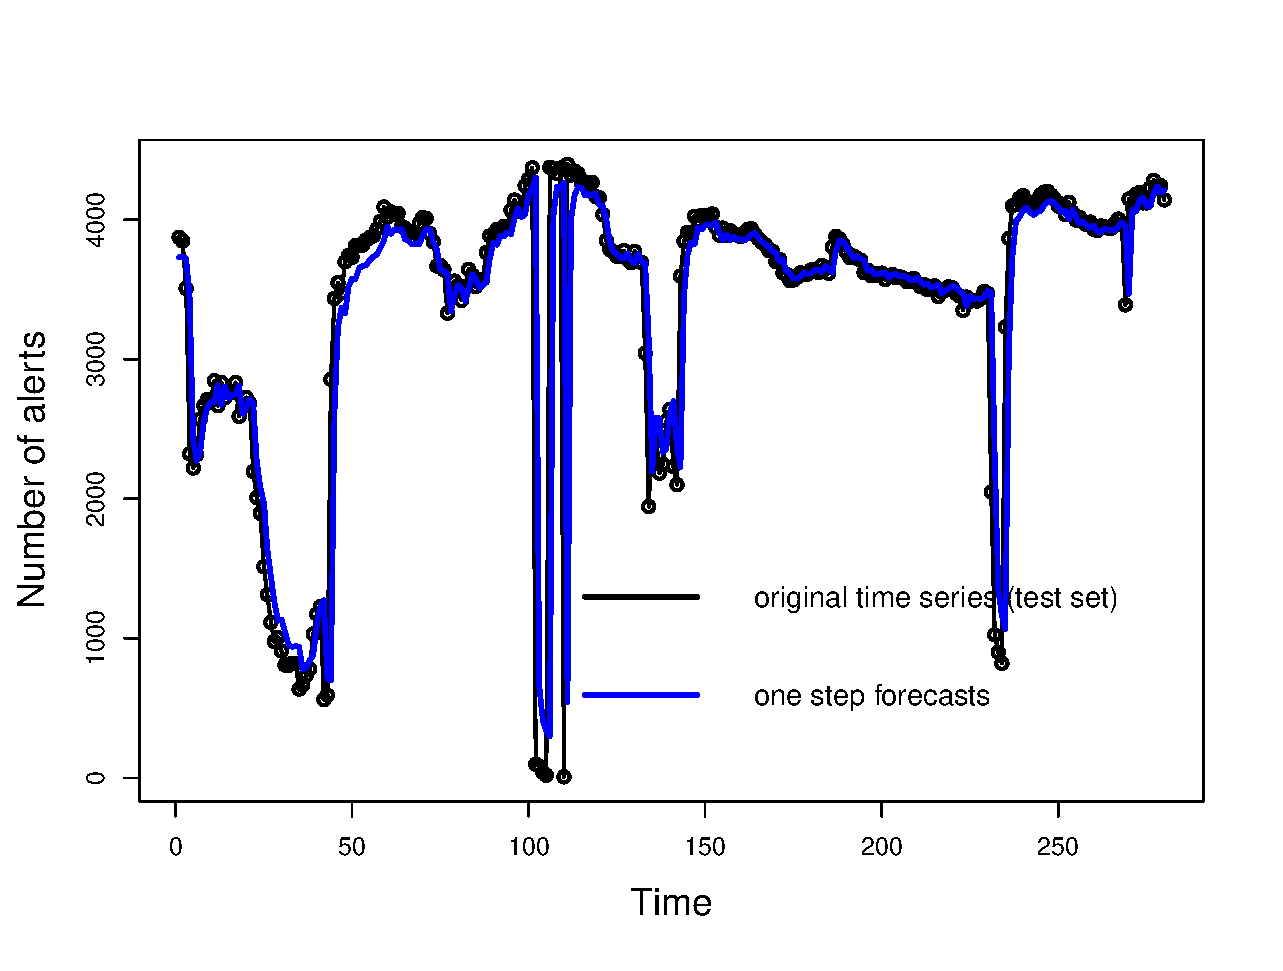
\includegraphics[width=0.7\textwidth]{images/item61_1step_forecasts_new.eps}
  \caption{Jednokroková predikcia atribútu: Kategória pokus o~prihlásenie.} 
  \label{fig:forecast_attempt_login}
\end{figure}

\begin{figure}[h]
  \centering
  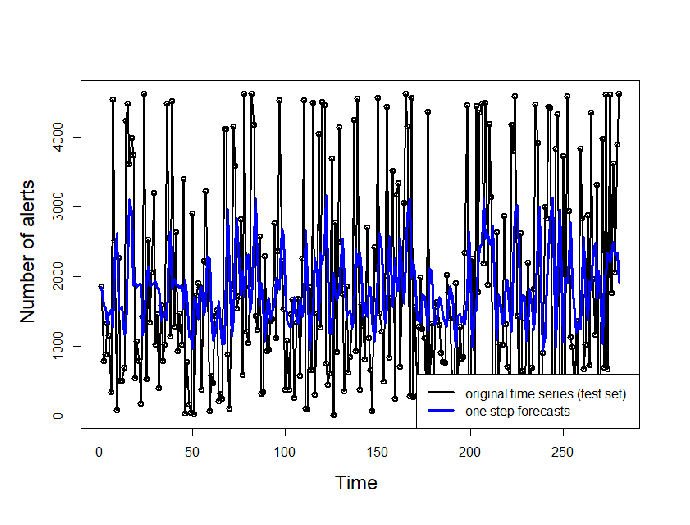
\includegraphics[width=0.7\textwidth]{images/item62_1step_forecasts_new.eps}
  \caption{Jednokroková predikcia atribútu: Kategória pokus o~prienik do~zariadenia. }
  \label{fig:forecast_attempt_exploit}
\end{figure}

\section{Výsledky}

% ------------- Seasonality  -----------------------------
Ako je uvedené vyššie, sezónnosť znamená cykly, ktoré sa pravidelne opakujú v~priebehu času. Vybrali sme metódy ETS a ARIMA, keďže dokážu odrážať sezónnosť údajov. Domnievame sa, že sezónnosť sa nemusí brať do~úvahy, pretože vzory v~údajoch (počet bezpečnostných udalostí) sa v~priebehu času neopakujú pravidelne (iba nepravidelne), ale závisia od~iných faktorov. Ako ukazujú výsledky, najlepšie hodnoty pre jednotlivé predpovede sa vždy dosahujú metódou v~oboch jeho formách, bez ohľadu na~sezónnosť. Z~tohto hľadiska môžeme konštatovať, že v~časových radoch založených iba na~celkovom počte útokov nehrá sezónnosť v~prognóze dôležitú úlohu.

% ------------- Rolling window  -----------------------------
Z našich výsledkov (tabuľka~\ref{tab:mase} a tabuľka~\ref{tab:avg_95}) vyplýva, že najúčinnejšie prístupy k~predikcii boli tie, ktoré používali techniku tzv. posuvného okna. Je to dobrý výsledok, pretože z~praktického hľadiska nie je potrebné uchovávať celý súbor údajov v~pamäti a nie je potrebné prispôsobovať modely, robiť výpočty a predikcie pomocou celej dátovej sady od~začiatku. Má zmysel nájsť primerane veľké okno, ktoré je zvyčajne oveľa kratšie ako dĺžka pôvodnej dátovej sady. To môže byť opäť výhodou, pokiaľ ide o~predikcie v~reálnom čase. V~našej štúdii sme považovali dĺžku okna za 80~\% mesačných údajov (časová jednotka - 30 min.) alebo 80~\% dvojmesačných údajov (časová jednotka - 60 min.).

%-------------------------------------------------------
% Research questions - discussion
%-------------------------------------------------------

\zaver

Mať prehľad o~kybernetickej situácii v~počítačovej sieti sa stáva dôležitejším aspektom pri zabezpečení organizácie. Vďaka prehľadu je možné proaktívne reagovať na~nové bezpečnostné, ale aj výkonnostné problémy. Táto práca sa venuje najmä kybernetickej situácii v~počítačovej sieti. Analyzujeme dáta získavané z~produkčných sietí formou bezpečnostných udalostí. Udalosti sú vytvárané sieťovými sondami, analýzou záznamov (logov) a pod. 

V práci sme sa zamerali na~povahu neustále generovaných a distribuovaných údajov čo vyžaduje časovo nenáročné operácie pre spracovanie údajov. Rozhodli sme sa použiť štruktúru časových radov. Pre distribúciu bezpečnostných údajov sme vybrali systém Apache Kafka. Údaje v~prvom kroku spracovávame manuálne, aby sme vybrali atribúty, pre ktoré je zaujímavé generovať časové rady. Viac o~výbere atribútov píšeme v~podkapitole~\ref{c1_metodologia}. Pri štúdii uvedenej v~parciálnych výsledkoch sme vybrali 21 atribútov, podľa ktorých boli vygenerované časové rady z~bezpečnostných udalostí. Ďalej sa v~práci venujeme predikcii časových radov a metrikám, pomocou ktorých dokážeme oprávnene ohodnotiť úspešnosť predikčných modelov. V~rámci štúdie uvedenej v~tretej kapitole sme bezpečnostné udalosti predikovali pomocou modelov ARIMA a exponenciálneho vyrovnávania aplikovaných na~časové rady. Analýzou časových radov sme dospeli k~testovaniu predikčných modelov s~alebo bez podpory pre sezónnosť. Ukázalo sa, že časové rady vzniknuté atribútom celkového počtu udalostí nevykazujú sezónnosť, naopak pre viac detailnejšie atribúty to môže byť inak.

V práci chceme dosiahnuť riešenie fungujúce v~nepretržitej prevádzke. Z~tohto dôvodu sme predikčné algoritmy analyzovali v~dvoch prístupoch, a to bez a s~posuvným oknom. Prístup posuvného okna je praktickejší pre požadované využitie vďaka menšej časovej a pamäťovej náročnosti. V~štúdii uvedenej v~tretej kapitole sa ukázalo, že použitím posuvného okna boli predikcie najúspešnejšie.

\bibliography{dp} %berie sa z~dp.bib
%
%
\prilohy

\textbf{Príloha A:} Zoznam publikácii \\
%\textbf{Príloha B:} P. Sokol, P. Pekarčik, and T. Bajtoš. Data collection and data analysis in honeypots and honeynets. In \textit{Proceedings of the Security and Protection of Information. University of Defence}, 2015. \\
\textbf{Príloha B:} P. Pekarčík, T. Kekeňák, P. Sokol, and T. Mézešová. Real-time processing of cybersecurity system data for attacker profiling. In \textit{2019 IEEE 15th International Scientific Conference on Informatics}, pages 207–212, 2019. \\
\textbf{Príloha C:} P. Pekarčík, A. Gajdoš and P. Sokol. Forecasting security alerts based on time series. In \textit{15th International Conference on Hybrid Artificial Intelligence Systems (HAIS’20)}, accepted, 2020.

\priloha{Zoznam publikácií autora}

\begin{enumerate}
\item P. Sokol, P. Pekarčik, and T. Bajtoš. Data collection and data analysis in honeypots and honeynets. In \textit{Proceedings of the Security and Protection of Information. University of Defence}, 2015.

\item P. Pekarčík. Spracovania kybernetických bezpečnostných údajov v~reálnom čase. In \textit{Zborník príspevkov zo~6. ročníka Jarnej internacializovanej školy doktorandov UPJŠ}, 2019.

\item E. Marková, P. Pekarčík, T. Bajtoš and P. Sokol. Malicious emails prevention system (MEPS). In \textit{International workshop: Data protection in real-time}, 2019.

\item P. Pekarčík, T. Kekeňák, P. Sokol, and T. Mézešová. Real-time processing of cybersecurity system data for attacker profiling. In \textit{2019 IEEE 15th International Scientific Conference on Informatics}, pages 207–212, 2019.

\item P. Pekarčík, A. Gajdoš and P. Sokol. Forecasting security alerts based on time series. In \textit{15th International Conference on Hybrid Artificial Intelligence Systems (HAIS’20)}, accepted, 2020.

% \item E. Marková, T. Bajtoš, P. Sokol, T. Mézešová and P. Pekarčík. Classification of malicious emails. In \textit{JOURNAL OF INTERNATIONAL STUDIES (JOIS)}, accepted, 2020.

\end{enumerate}

\newpage

%\setlength{\voffset}{0.5in}
%\setlength{\hoffset}{1in}

%\refstepcounter{chapter}%
%\addcontentsline{toc}{section}{\protect\numberline{\thechapter}Data collection and data analysis in honeypots and honeynets.}
%\includepdf[pages=-,fitpaper=true]{priloha/clanok-DataCollection1.pdf}


\setlength{\voffset}{0in}
\setlength{\hoffset}{0in}

\refstepcounter{chapter}%
\addcontentsline{toc}{section}{\protect\numberline{\thechapter}Real-time processing of cybersecurity system data for attacker profiling.}
\includepdf[pages=-,fitpaper=true]{priloha/clanok-Profiling.pdf}

\refstepcounter{chapter}%
\addcontentsline{toc}{section}{\protect\numberline{\thechapter}Forecasting security alerts based on time series.}
\includepdf[pages=-,fitpaper=true]{priloha/clanok-HAIS.pdf}

\end{document}